\documentclass[10pt,letterpaper]{article}
\usepackage[margin=.85in]{geometry}
\usepackage[T1]{fontenc}
\usepackage{lmodern,microtype,amsmath,amssymb}
\usepackage{textcomp,fvextra,graphicx}
\usepackage{booktabs,array,longtable,tabularx,enumitem}
\usepackage{xcolor,tikz,hyperref,xurl,fancyhdr,needspace}
\usetikzlibrary{arrows.meta,positioning,calc}
\definecolor{ink}{HTML}{183448}
\definecolor{accent}{HTML}{245D73}
\definecolor{pale}{HTML}{EFF5F7}
\hypersetup{colorlinks=true,linkcolor=accent,urlcolor=accent,citecolor=accent,
  pdftitle={TriAlign Technical Design and Research Notes},
  pdfauthor={Jonathan Ma and Jiatong Gao}}
\setlist[itemize]{leftmargin=1.6em,itemsep=.25em,topsep=.4em}
\setlist[enumerate]{leftmargin=1.9em,itemsep=.35em,topsep=.4em}
\setlength{\parskip}{.35em}
\setlength{\parindent}{0pt}
\setlength{\emergencystretch}{2em}
\renewcommand{\arraystretch}{1.18}
\newcolumntype{L}[1]{>{\raggedright\arraybackslash}p{#1}}
\newcolumntype{Y}{>{\raggedright\arraybackslash}X}
\newcommand{\code}[1]{\texttt{\detokenize{#1}}}
\newcommand{\pathcode}[1]{\nolinkurl{#1}}
\newcommand{\planned}{\textit{Proposed design.}}
\newcommand{\research}{\textit{Research note; adaptation not yet implemented or evaluated.}}
\pagestyle{fancy}
\fancyhf{}
\fancyhead[L]{\small\textcolor{ink}{TriAlign technical design}}
\fancyhead[R]{\small November 2026}
\fancyfoot[C]{\thepage}
\setlength{\headheight}{14pt}
\setcounter{tocdepth}{2}
\title{\textcolor{ink}{TriAlign Technical Design}\\[.4em]
  \large An Agent for Clinically Meaningful Comparison of Eligibility Criteria\\
  \normalsize Architecture, Dataset, Pair Semantics, Interface Concepts, and Research Notes}
\author{Jonathan Ma \and Jiatong Gao}
\date{Revised November 7, 2026}

\begin{document}
\maketitle
\begin{abstract}
TriAlign has two tasks: identify candidate criterion pairs across trials, then
compare their clinical relationships using structured constraints, learned
representations and contextual reasoning. This document defines what constitutes a clinically meaningful criterion relationship,
how source evidence and normalization are retained, how an agent selects and
reconciles comparison tools, and how a clinician could inspect and correct a
result. The frozen criterion release contains 3,537 records from 100 trials.
The first development pair-review release preserves 75 decisions, including
67 clean comparisons and eight queued cases. A functional local comparison interface and bounded agent runtime are implemented.
Fine-tuned models and independent clinical evaluation remain subsequent deliverables.
\end{abstract}

\newpage
\tableofcontents
\newpage

\section{Motivation}
\label{sec:motivation}

\subsection{The Clinical Problem}
An eligibility criterion determines what characteristics a patient must have to be included in a clinical trial.
Two rules can reuse the same terminology while admitting different people, ie "age $\ge$ 18 years" vs "age < 18 years" have similar vocabulary and disjoint allowed age ranges. Conversely,
an abbreviation and an expanded term may express the same rule with limited word overlap. TriAlign is intended to pull seemingly similar criteria apart when
clinical investigators, protocol designers, and research coordinators compare
protocols.

The intended clinician-facing workflow compares the eligibility requirements
of Trial A and Trial B. Criterion-to-criterion comparison is the computational
unit underneath that view: retrieve rules about the same clinical concept,
inspect their operational differences, and record an evidence-supported
relationship. Individual-criterion search remains useful as a separate entry
point. Potential applications include identifying precedent during
protocol design, comparing amendments, documenting harmonization decisions,
and inspecting whether superficially similar study populations are defined
by materially different criteria. These applications motivate the system;
their clinical benefit must be measured rather than assumed.

TriAlign does not determine an individual patient's eligibility, recommend a
treatment, estimate recruitment yield without patient data, or establish
causal transportability. A criterion-level comparison is not a claim that
two complete protocols recruit the same population: their remaining rules,
sites, ascertainment practices, and treatment settings may differ.

\subsection{Trial comparison workflow}
\label{sec:trialworkflow}
The clinician selects two trials, uses Modern AutoCrit to extract and
structure their eligibility criteria, reviews the extracted records, and
imports the resulting criteria files into TriAlign. TriAlign is intended to
align comparable requirements and display their relationships, differences,
source evidence, unresolved cases and requirements without a supported
match. Figure~\ref{fig:trialworkflow} is the same diagram used in the progress
presentation.

\begin{figure}[htbp]
\centering
\resizebox{.98\linewidth}{!}{%
  \IfFileExists{docs/figures/trial_comparison_workflow.tex}
    {% Shared editable diagram used by the progress deck and technical document.
\begingroup
\definecolor{wfWine}{HTML}{9B1C2B}
\definecolor{wfOrange}{HTML}{D97800}
\definecolor{wfInk}{HTML}{302F2D}
\definecolor{wfPale}{HTML}{FFF9F5}
\hyphenpenalty=10000
\exhyphenpenalty=10000
\begin{tikzpicture}[
  font=\sffamily\fontsize{10}{12}\selectfont,
  wfbox/.style={draw=wfInk!55,line width=.65pt,rounded corners=2pt,
    fill=white,text=wfInk,align=center,text width=2.8cm,
    minimum height=2.5cm,inner sep=6pt},
  wfsystem/.style={wfbox,draw=wfWine,fill=wfPale},
  wfarrow/.style={-{Latex[length=2.2mm]},draw=wfWine,line width=.9pt}
]
\node[wfbox] (trials) at (0,0) {
  \textbf{1. Select trials}\\[4pt]
  Clinician chooses\\Trial A + Trial B
};
\node[wfsystem] (extract) at (3.65,0) {
  {\color{wfWine}\textbf{2. Extracted}}\\
  {\color{wfWine}\textbf{criteria}}\\[4pt]
  Modern AutoCrit or\\another compatible source
};
\node[wfbox] (handoff) at (7.3,0) {
  \textbf{3. Review}\\\textbf{and import}\\[4pt]
  Reviewed files\\Source evidence
};
\node[wfsystem] (compare) at (10.95,0) {
  {\color{wfWine}\textbf{4. TriAlign}}\\[4pt]
  Identify pairs\\Compare clinical\\relationships
};
\draw[wfarrow] (trials) -- (extract);
\draw[wfarrow] (extract) -- (handoff);
\draw[wfarrow] (handoff) -- (compare);

\node[draw=wfOrange,line width=.8pt,rounded corners=2pt,
  fill=white,text=wfInk,align=center,text width=13.3cm,
  minimum height=1.65cm,inner sep=7pt] (view) at (5.475,-3.05) {
  \textbf{Clinician's Trial A vs Trial B comparison}\\[4pt]
  Matched rules: equivalent, stricter, overlapping or conflicting\\
  Unmatched or unclear rules, with source-linked explanations
};
\draw[wfarrow] (compare.south) -- (10.95,-1.9)
  -| (view.north);
\node[text=wfWine,font=\sffamily\fontsize{9.5}{11}\selectfont,
  anchor=south] at (7.8,-1.8)
  {Two tasks build the trial view};
\end{tikzpicture}
\endgroup
}
    {\input{figures/trial_comparison_workflow.tex}}%
}
\caption{Intended workflow: a clinician compares two trials through
source-grounded criterion comparisons. A relationship between two rules
does not establish a relationship between the complete trial populations.
Candidate-pair identification and the local comparison interface are implemented;
trained components and direct extraction integration remain planned.}
\label{fig:trialworkflow}
\end{figure}

The encoder retrieves potentially corresponding criteria; the relationship
component and contextual review determine how selected pairs compare.
Criterion-pair labels train and evaluate those components. The current trial view assembles candidate-pair results. Group-level alignment
across different extraction granularities is deferred research
(Section~\ref{sec:deferrednovelty}). A retrieved neighbor is not automatically
a semantic match, and no match found is not proof that a requirement is
absent from the other protocol. This workflow does not yet define a validated
single whole-trial similarity score. A future combined application could
remove the manual file handoff while retaining the review checkpoint and
separate component modes (Section~\ref{sec:combinedtool}).

\subsection{Two tasks: pair identification and relationship comparison}
\label{sec:twotasks}
\textbf{Use these terms consistently throughout the project.} TriAlign identifies
candidate counterparts between trials and then determines their clinical
relationships. Modern AutoCrit is the upstream extraction component in the
demo; TriAlign also runs independently on imported criterion records. Extraction,
pair identification and relationship comparison are distinct operations.

\begin{longtable}{L{.20\linewidth}L{.36\linewidth}L{.35\linewidth}}
\toprule Task & Question and output & Current and planned methods\\\midrule
\endhead
1. Pair identification & Which criteria across Trial A and Trial B should be compared? Output ranked candidate pairs with source IDs. & TF--IDF plus entity priority in the current demo; Jiatong's TF--IDF, MPNet and BioLORD backends establish baseline pair-similarity rankings. A trained clinical encoder is planned.\\
2. Relationship comparison & How do a selected pair's allowed populations relate? Output a directional/categorical relationship, evidence and uncertainty or an unresolved review disposition. & Exact tools and contextual LLM judge/critic in the current demo. A separately trained ordered relationship head is planned.\\\bottomrule
\end{longtable}

For example, Task 1 identifies ``age at least 18'' and ``age at least 21'' as
candidate counterparts. Task 2 determines that the second inclusion rule is
more restrictive within a shared age frame. Candidate identification does not
certify equivalence: even ``age at least 18'' versus ``age below 18'' may be
important counterparts because their conflict is useful to expose. Relevance
for comparison and clinical equivalence must therefore be distinguished in
annotation and training.

In this document, \textbf{baseline pair-similarity methods} refers to TF--IDF,
MPNet and BioLORD as used to score/rank candidate pairs. TF--IDF is a lexical
method; MPNet and BioLORD supply embeddings for similarity scoring. None is
an extraction model in this workflow. The term \textbf{relationship model}
refers to a classifier/head that predicts the clinical relationship for an
ordered A/B input; a symmetric similarity score alone does not supply the
A-more-restrictive versus B-more-restrictive distinction. Prefer these terms
to the ambiguous phrase ``pair model'' without qualification.

Reviewed pairs support evaluation and potential training of both tasks, with
separate target definitions. Evaluate pair identification by whether relevant
counterparts appear in the ranked candidates; evaluate relationship comparison
on the same fixed reviewed pairs across methods, so retrieval misses do not
confound classifier performance. In end-to-end evaluation, account for both
missed counterparts and wrong relationships. The teammate's baseline ranking
work is part of Task 1 and remains required for evaluating an improved encoder.
When a user supplies exactly two criteria, Task 1 is already supplied and only
Task 2 needs to run; the trial-versus-trial interface requires both tasks.

\subsection{Why textual similarity is insufficient}
The clinical meaning of a rule depends on more than its entity name.
\begin{longtable}{L{.20\linewidth}L{.34\linewidth}L{.37\linewidth}}
\toprule Dimension & Illustrative difference & Comparison implication\\\midrule
\endhead
Polarity & Require a condition versus exclude that condition. & Interpret the allowed population before using numerical or categorical agreement.\\
Threshold and boundary & Age $\geq18$ versus $>18$. & A one-point boundary changes equivalence and containment.\\
Units and references & Absolute bilirubin concentration versus a multiple of ULN. & Equal numbers need not be comparable quantities.\\
Time and anchor & Event in the previous six months versus six months after treatment. & Duration, direction, and reference event must agree.\\
Repetition & A single observation versus two observations on separate occasions. & An identical threshold can encode a stronger evidentiary requirement.\\
Disease specificity & Active disease, previous disease, anatomical site, stage, or severity. & Ontological similarity alone does not establish equal eligibility.\\
Exceptions & Other malignancy excluded except specified cured cancers. & Removing the exception reverses the interpretation of an allowed subgroup.\\
Boolean scope & $A\land B$ versus $A\lor B$, possibly inside a larger clause. & Independent atoms must retain their branch conditions.\\\bottomrule
\end{longtable}

An embedding score can be useful for finding a likely comparison without being
a valid clinical relationship score. In particular, cosine similarity is
symmetric, whereas ``A is more restrictive than B'' is directional. A high
cosine score therefore cannot, by itself, select a directional label or prove
equivalence.

\subsection{Research questions and hypotheses}
Three questions we.re interested in are:
\begin{enumerate}
\item Which phenomena produce false-high similarity for clinically different
rules, or false-low similarity for equivalent rules, in general and biomedical
encoders?
\item Does supervision from reviewed positives, ordinary negatives, hard
negatives, and ordered anchors improve held-out retrieval and relationship
prediction?
\item Does selective tool routing improve evidence support, calibration,
reviewer effort, latency, or cost relative to an LLM-only judge and an
always-run fixed chain?
\end{enumerate}

\section{Eligibility Criteria Dataset}
\label{sec:data}

\subsection{Modern AutoCrit and the upstream handoff}
Modern AutoCrit produces the source records used by TriAlign. It accepts an
NCT identifier, protocol text, or a protocol PDF; locates eligibility content;
distinguishes inclusion from exclusion; extracts atomic constraints; and
preserves the parent statement and local context. Extraction records include
clinical fields, source identifiers, protocol versions, validation findings,
and review status. TriAlign consumes reviewed outputs rather than replacing
this extraction system. Criterion review corrects segmentation, polarity, measurement fields,
normalization, and scope.

\subsection{Current frozen release and historical counts}
\begin{table}[htbp]\centering
\begin{tabularx}{\linewidth}{L{.30\linewidth}Y}\toprule
Release property & Verified value or source\\\midrule
Dataset version & \code{trial100_v1}\\
Source workbook & \pathcode{data/trial100_v1.xlsx}, sheet \code{Human Review}\\
Frozen snapshot & \pathcode{data/processed/trial100_v1.parquet}\\
Manifest & \pathcode{data/processed/trial100_v1.parquet.manifest.json}\\
Retained criteria / trials & 3,537 / 100\\
Review status & 3,537 corrected; zero pending\\
Export readiness & All retained rows export-ready; zero recorded validation issues or readiness blockers\\
Schema version & \code{0.1.0}\\
Pair labels & Not included in the criterion release\\\bottomrule
\end{tabularx}
\caption{Current release facts are drawn from the frozen manifest. A review-status
flag is distinct from a pair label or a calibrated confidence estimate.}
\end{table}

The cohort design
in the proposal is 50 oncology and 50 cardiovascular trials. Therapeutic-area
evaluation will use an explicit trial-level mapping; that design statement
is not a verified per-row therapeutic-area annotation in the manifest.

The initial extraction had 3,145 candidates. Splitting, correction, and removal
changed the number of retained records. The October 20 proposal milestone
reported approximately 2,900 reviewed cases and a remaining uncertainty queue.
Those historical workload figures are not the denominators for v1 evaluation.
Use the frozen manifest and saved split files for every reported result.

\subsection{Record schema and evidence hierarchy}
\begin{longtable}{L{.22\linewidth}L{.40\linewidth}L{.29\linewidth}}
\toprule Field group & Representative fields & Technical use\\\midrule
\endhead
Identity and lineage & \code{criterion_id}, \code{row_id}, \code{trial_id}, \code{parent_statement_id}, \code{origin_criterion_id} & Stable joins, split membership, split-parent lineage, and audit history.\\
Source evidence & \code{source}, \code{source_excerpt}, \code{parent_statement}, \code{surrounding_context} & Human inspection, evidence citations, and scope reconstruction.\\
Clinical predicate & \code{criterion_type}, \code{domain}, \code{entity}, \code{comparator}, \code{value}, \code{unit}, \code{value_kind}, bounds and inclusivity & Reconstruct the stated constraint before interpreting its eligibility effect.\\
Context and logic & \code{negated}, \code{temporal}, \code{repetition}, \code{qualifier}, \code{logical_operator}, \code{boolean_group_id}, atom indices/counts & Retain conditions and connections among atoms; flat fields alone do not certify a complete Boolean tree.\\
Normalization & Raw and normalized entity/value/unit fields; normalized bounds; \code{reference_type}, \code{reference_multiplier}; methods/status/confidence & Controlled matching while preserving source-grounded values and normalization provenance.\\
Protocol provenance & \code{source_uri}, \code{source_version}, \code{source_retrieved_at}, \code{protocol_hash}, \code{source_id} & Identify the exact source snapshot rather than silently following a changed registry page.\\
Review and release & \code{review_status}, \code{export_ready}, issue/blocker lists, review-method metadata & Admission to the release and traceability of subsequent corrections.\\\bottomrule
\end{longtable}

The evidence hierarchy is the protocol wording and its governing context,
followed by the reviewed structured interpretation and normalization. When an atom and its parent appear
inconsistent, the system should expose the conflict and request adjudication.
Opening a current registry link does not establish that its wording matches
the version originally extracted.

\subsection{Normalization and serialization}
Terminology normalization supports retrieval across abbreviations, spelling
variants, and aliases. It must preserve disease stage, severity, anatomical
site, assay, and treatment context. A normalization dictionary should carry
its own version and provenance, and proposed synonym merges should be evaluated
for both false merges and missed aliases. A method/status field can describe
normalization without establishing that its numeric confidence is calibrated.

Physical-unit normalization and reference normalization are different.
``Bilirubin $\leq1.5\times\mathrm{ULN}$'' uses \code{reference_type=ULN}
and multiplier 1.5. ULN is not a physical concentration unit. A local upper
limit can vary by assay or institution, so reference-relative and absolute
thresholds require explicit reference information before conversion.
Likewise, systolic/diastolic notation does not authorize inferring an AND/OR
relationship that the source did not specify.

The source's clinical and normalization fields are retained in the snapshot.
Schema loading standardizes missing values, Boolean fields, issue lists, and
the casing of selected categorical status fields. Because Parquet requires
homogeneous column types, the mixed \code{value}, \code{value_raw}, and
\code{value_normalized} columns use manifest-declared JSON scalar encoding.
The project loader decodes these columns, preserving numeric values,
categorical strings such as ``001'', and Booleans. Numerical bounds remain
typed numeric columns. Direct consumers of Parquet must read the manifest;
they must not interpret JSON scalar text as already-decoded clinical values.

\subsection{Release integrity and changes after freezing}
The release records the source and Parquet hashes, schema version, criterion-ID
fingerprint, creation time, Git revision, and exporter/script hashes. The
export was reopened through the project loader and reconciled record by
record against source-derived records. These checks establish serialization
integrity, not independent clinical certification of every interpretation.

A correction after freezing creates a new dataset version, an explicit change
record, and a regenerated manifest. Existing pair records must continue to
identify the corpus version against which they were labeled. A source edit
must not silently change an already-published training or test example.
Shared public-source subsets should retain this provenance and an intended-use
statement. Sharing the criterion corpus with the group mentioned in the
October presentation feedback must not expose protected TriAlign test labels.

\subsection{Optional external data}
Chia is an annotated eligibility-criteria corpus with entity, relation, and
scope representations \cite{chia}. It may supply external terminology or
logical-complexity examples. Its annotations do not directly provide
TriAlign's eight pair relationships. Any use requires an explicit schema
mapping, license/source review, overlap checks, and separate reporting; it
must not be silently mixed into the v1 benchmark.

\section{Clinical Pair Definitions}
\label{sec:pairs}

\subsection{The ordered comparison unit}
A pair contains two reviewed criteria, A and B, normally from different
protocols, together with their corpus versions, trial/criterion identifiers,
source excerpts, parent context, structured fields, and sampling provenance.
The input order is part of the task. An unordered pair-group identifier can
deduplicate cases and hold reversed views together, while an ordered pair
identifier or orientation field preserves the direction of prediction.
Mirrored cases must not become independent examples across train and test.

Criterion approval establishes that one record represents its source rule.
It does not establish a relationship to any other criterion. Pair labeling is
a second review with its own evidence, uncertainty, and adjudication record.
The following formalization is an operational draft of the labeling contract;
JM must approve the final guide before benchmark labels are frozen.

\subsection{Allowed populations and comparability}
Let $U_{\gamma}$ be a common comparison universe under explicit context
$\gamma$, including the measurement, population, temporal anchor, and branch
scope. Let $P_c(x;\gamma)$ be the clinical predicate stated by criterion $c$,
with its internal negation and exceptions already interpreted. The
criterion-level allowed set is
\[
 S(c;\gamma)=
 \begin{cases}
 \{x\in U_{\gamma}:P_c(x;\gamma)\}, & c\text{ is an inclusion rule},\\
 U_{\gamma}\setminus\{x:P_c(x;\gamma)\}, & c\text{ is an exclusion rule}.
 \end{cases}
\]
An internal negation is applied inside $P_c$; inclusion/exclusion is applied
once outside it. A categorical value ``absent'' and a negation flag must not
accidentally invert a predicate twice. Record their combined interpretation
before comparing sets.

Set operations are meaningful only after establishing a common operational
frame. Age and platelet count can both restrict a person, but this does not
make their comparison a useful ``partial overlap'' label. First determine
conceptual comparability. Related measurements such as serum creatinine and
estimated glomerular filtration rate may require a clinical mapping that is
not available; terminology similarity alone is insufficient.

\subsection{Eight relationship labels}
For comparable, interpretable criteria, write $S_A=S(A;\gamma)$ and
$S_B=S(B;\gamma)$.
\begin{longtable}{L{.23\linewidth}L{.39\linewidth}L{.29\linewidth}}
\toprule Label & Operational definition & Illustrative pair\\\midrule
\endhead
Equivalent & $S_A=S_B$, including applicable scope and exceptions. & Inclusion age $\geq18$ versus age $\geq216$ months after a valid age-unit conversion.\\
A more restrictive & $S_A\subsetneq S_B$. & A: inclusion age $\geq21$; B: age $\geq18$.\\
B more restrictive & $S_B\subsetneq S_A$. & The preceding pair reversed.\\
Partial overlap & Nonempty intersection, with neither set containing the other. & Inclusion ages 18--65 versus 50--80, all endpoints inclusive.\\
Contradictory or disjoint & $S_A\cap S_B=\varnothing$ in the common operational frame. & Inclusion age $\geq18$ versus age $<18$. This does not claim that the complete trials are mutually exclusive.\\
Related but not comparable & A meaningful clinical relationship exists, but a defensible shared constraint representation or mapping is unavailable. & Renal-function rules expressed through different measures without a supported conversion.\\
Unrelated & No meaningful direct clinical comparison for this task. & An age threshold versus an unrelated laboratory requirement.\\
Ambiguous & Missing or conflicting evidence prevents a defensible choice among the relationships. & A truncated rule whose polarity or governing exception cannot be established.\\\bottomrule
\end{longtable}

The distinction between ``related but not comparable'' and ``ambiguous'' is
important. In the first case, the concepts are understood but the relationship
cannot be ordered in the available representation. In the second, the
meaning or relevant context of the input itself is insufficient. Annotators
should record the reason, not force uncertain cases into an ordinary
negative class. Empty or internally inconsistent allowed sets also require
an explicit inconsistency disposition rather than a misleading containment
label based on the mathematical empty-set convention.

\subsection{Labeling decision procedure and worked safeguards}
\begin{enumerate}
\item Confirm the source version and that both records are eligible for pair
review. Inspect parent statements and any linked atoms needed for scope.
\item Identify the clinical quantities, anatomical/clinical context, applicable
population, measurement method, temporal window, and exceptions.
\item Classify clear unrelatedness, related non-comparability, or unresolved
ambiguity. Otherwise establish the common comparison frame.
\item Translate each rule into its criterion-level allowed predicate. Validate
units/references, boundary inclusivity, internal negation, and eligibility role.
\item Determine equality, proper containment, intersection, or separation.
Record a concise evidence-supported explanation and any assumptions.
\item Reverse A and B as a consistency check. Only the two restrictive labels
swap; symmetric labels remain unchanged.
\end{enumerate}

For example, inclusion ``age $\geq18$'' and exclusion ``age $\geq18$'' are
not equivalent: the latter allows ages below 18 under the simplified common
age universe. Similarly, changing a negation flag does not prove disjointness
unless the complete predicates are complements. The allowed set for
$\neg(\mathrm{age}\geq65)$ overlaps the set for $\mathrm{age}\geq18$.
Different lookback windows can change the relationship even when entity,
threshold, and units match. A single atom from $A\land B$ is not an
independent exclusion unless its conjunction condition remains explicit.

\subsection{Annotation record and review protocol}
\begin{longtable}{L{.26\linewidth}L{.66\linewidth}}
\toprule Annotation component & Required content\\\midrule
\endhead
Identity & Ordered pair ID, unordered pair-group ID, corpus version, A/B criterion IDs and trial IDs.\\
Evidence & Source excerpts, parent/context references, source versions/links, and field-level differences used by the reviewer.\\
Sampling & Every candidate-generation method that selected the pair, retrieval model/version and rank/score, phenomenon tags, and natural/constructed flag.\\
Decision & Eight-class label, direction, rationale, assumptions, source-ambiguity reason, reviewer uncertainty, and review status.\\
Adjudication & Reviewer identity, initial independent decisions when available, final adjudicator, revision history, and unresolved disposition.\\
Evaluation control & Family/group IDs, split, annotation-guide version, duplicate/variant links, and whether the case was used for development or demonstration.\\\bottomrule
\end{longtable}

JM owns pair definitions, construction, labeling, adjudication, and evaluation
changes. JG consumes the approved development records for software and model
work and does not redefine gold labels to fit outputs. Independent second
annotation of a documented subset is desirable; if a second reviewer is
available, preserve the initial disagreement and JM's adjudication rather
than reporting only the consensus. The guide should be piloted and revised
before the held-out benchmark is locked. Model suggestions and similarity
scores should be hidden during an independent gold-labeling round where
feasible, reducing anchoring on the method being evaluated.

\subsection{Family splits and pair sampling}
Map trials to families before candidate generation. Related protocols,
amendments, template-derived duplicates, and constructed variants must stay
in one partition. A 70/15/15 family allocation is a starting configuration,
not a guarantee of balanced criteria or relationship classes. Audit the
actual family counts, oncology/cardiovascular composition, domains, and
pair opportunities; record a fixed seed and the complete mapping.
Missing split assignments must cause a pair-generation failure or explicit
rejection, not silent inclusion in the known side's partition.

Candidate pools should combine canonical-entity matches, nearest neighbors
from multiple encoders, lexical neighbors, random controls, and targeted
clinical phenomena. Record overlapping sampling memberships instead of
letting whichever generator ran first erase the others. Natural pairs measure
behavior in the observed corpus; constructed paraphrases and controlled
threshold/negation changes test diagnostic capabilities and are reported
separately. Random controls mainly provide easy unrelated cases and must not
dominate a benchmark intended to test subtle clinical differences.

\subsection{Pair construction contract and development pilot v1}
\label{sec:pairpilot}
The operational annotation guide is contained in Appendix~\ref{sec:labelingcontract},
revised to \pathcode{pair-guide-0.2} on November 7, 2026. The original pilot
construction guide 0.1 is retained separately; decisions record the guide
actually used rather than silently changing construction metadata.
The guide applies the eight labels and comparison
gates above to an ordered A/B example. Hash A then B for the ordered ID and
sorted criterion IDs for the unordered group ID. Presentation direction is
seeded independently of any presumed relationship. The pilot stores one
direction per group; reverse-direction checks must exchange only the two
restrictive labels. Predictions, random-control membership and structured
differences never supply gold labels.

\textbf{Development reservation before final splitting.} Family mappings
had not yet been audited when the pilot was constructed. The initial pilot therefore reserves twenty
seed-selected trials for development rather than claiming a leakage-resistant
train/test split. All reserved trials, and any related families discovered
later, must be excluded from the final held-out test set. Merely inspecting
a case while refining the guide counts as development exposure. The complete
reservation list is saved in the pilot manifest. Audit family, template and
duplicate links before freezing the remaining partitions and performing
full-scale mining. The existing generic pair generator remains scaffolding;
it is not the source of this pilot or an approved final split contract.

\textbf{Sampling release.} The original pilot used this generator command:
\begin{verbatim}
python scripts/build_pair_pilot.py
\end{verbatim}
That builder is absent from the current checkout and must be restored before
resampling. At construction it verified the frozen Parquet hash and checked unique
IDs and reviewed statuses. Seed 20261104 selects the development pool and
presentation order. The output is
\pathcode{data/processed/pair_pilot_v1/}; an existing directory is rejected
instead of overwritten. Use \pathcode{--output} to make a new version.
The 75 natural cross-trial pairs comprise 25 same-entity pairs with structured
differences, 25 further same-entity pairs, 15 lexical neighbors and 10 random
controls. Literal entity matching normalizes case and whitespace only.
Lexical sampling uses source-token Jaccard similarity of at least 0.25
within the same domain and ranks eligible candidates by that score.
ASCII operators and numbers are retained as tokens; Unicode inequality-token
support is a limitation of the initial heuristic. This is a sampling heuristic,
not a clinical similarity score. Cap reuse at three pairs per criterion and
four per unordered trial pair. Quota shortfalls cause failure rather than
silent changes to the sampling design.

Store every qualifying method membership and the primary quota-filling
method. Membership denotes eligibility under a rule, not independent
selection or a known inclusion probability. The enriched convenience sample
cannot estimate corpus-wide relationship prevalence. It contains no synthetic
edits or embedding-mined candidates; add those as separately identified
sampling conditions after the teammate's baseline integration is reviewed.

\textbf{Review artifacts and acceptance.} The JSONL packet stores full A/B
records, source and parent evidence, available context and provenance,
ordered/group IDs, corpus and guide versions, sampling information, and blank
review fields. The labeling workbook separates review fields from source evidence. The
retired Markdown packet is recoverable from the source archive in this document. The manifest records corpus, source-manifest and generator hashes,
seed, development reservations, counts and output checksums. Verify 75 unique
unordered pairs, cross-trial membership, quotas, reuse caps, empty labels and
deterministic regeneration before review. These checks validate construction,
not clinical correctness or label balance.

Keep the sampling release immutable. Save reviewer decisions in a separate
versioned annotation file keyed by ordered ID, using the blank review object
as its template. Require a supported common frame, cited evidence, rationale,
assumptions, reviewer identity, low/medium/high reported uncertainty and status;
an adjudicated record requires a final label. Preserve unresolved questions,
independent initial decisions and adjudication history. Source corrections
require a new corpus release and pair migration rather than edits to the
frozen snapshot. Review the pilot before expanding the pool; revise the guide,
audit family exclusions, and only then lock the held-out benchmark.

\subsubsection{Guide revision and initial family audit}
Guide 0.2 clarifies atom versus parent scope, inclusion/exclusion Boolean
logic, conditional exceptions, measurement anchors, ULN conversions,
consent capability versus completion, and the distinction between ambiguity
and unavailable operational mappings. The original draft is preserved as a
historical round. The current frozen development review is documented in
Section~\ref{sec:pairfreeze}; reviewer identity and revision history remain
explicit, and independent clinical validation is still a separate gate.

The November 7 family audit reconciles all 100 trials and screens all 4,950
trial pairs using archived eligibility and registry identity/lineage evidence.
The 22 prioritized text-similarity pairs do not supply a supported in-cohort
family merge. The map therefore has 100 provisional current families, not
100 proven independent studies. Three verified external links capture
PREVAIL/CAP2, separately registered ZUMA-2 cohorts, and participant follow-up.
Clinical-family membership and participant-overlap split groups are recorded
separately. Full methods and source evidence are in
Appendix~\ref{sec:familyaudit}.

Unnamed linked studies for the master-screening trial NCT05419375 and
rollover trial NCT07172919 remain unresolved. Retaining their conservative
exclusions together with the pilot reservations excludes 21 current trials
and 841 criteria from final held-out testing. No final partition assignments
have been created. A scale-up split artifact must consume both
\pathcode{split_group_by_trial} and
\pathcode{holdout_excluded_trial_ids} from
\pathcode{data/processed/family_audit_v1/family_mapping.json}.
The current generic split CLI does not enforce this map or reservations;
integrate and validate that contract before mining a larger benchmark.

\section{Agentic Architecture}
\label{sec:agent}

\subsection{Runtime workflow and tool contracts}
The system has an offline data/model workflow and an online comparison
workflow. Offline work freezes the corpus and splits, builds candidate pools,
collects labels, trains models when justified, selects policies on development
data, and prepares versioned indexes. Online inference uses frozen weights
and versions; reviewer corrections enter an audit log and a later offline
release rather than silently changing a running model.

\begin{figure}[htbp]\centering
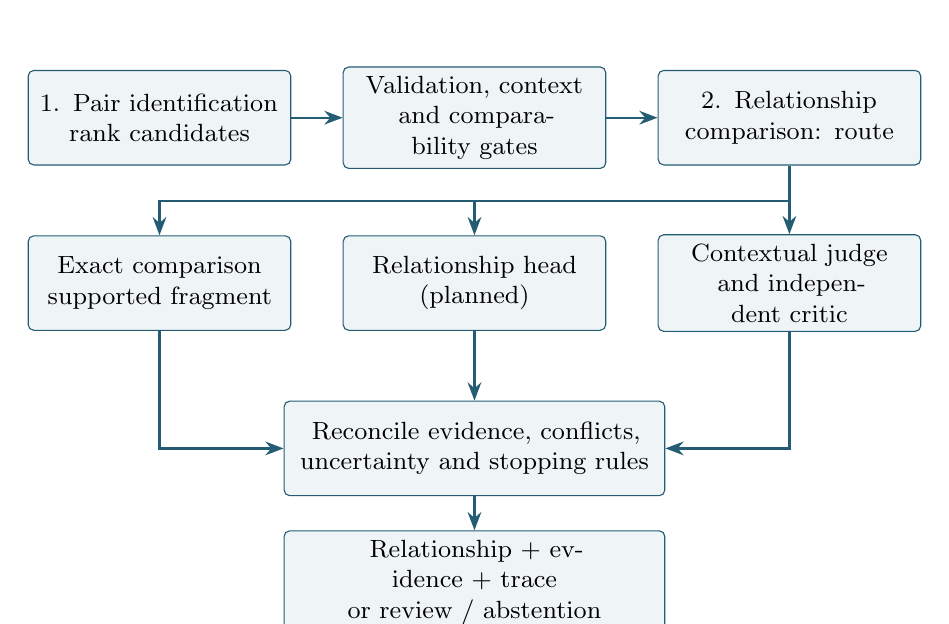
\begin{tikzpicture}[
  box/.style={draw=accent,rounded corners=2pt,fill=pale,align=center,
    text width=31mm,minimum height=12mm,font=\small},
  arrow/.style={-{Stealth},thick,draw=accent}]
\node[box](input) at (0,0) {1. Pair identification\\rank candidates};
\node[box](gate) at (4,0) {Validation, context\\and comparability gates};
\node[box](router) at (8,0) {2. Relationship\\comparison: route};
\node[box](exact) at (0,-2.1) {Exact comparison\\supported fragment};
\node[box](encoder) at (4,-2.1) {Relationship head\\(planned)};
\node[box](llm) at (8,-2.1) {Contextual judge\\and independent critic};
\node[box,text width=46mm](reconcile) at (4,-4.2) {Reconcile evidence, conflicts,\\uncertainty and stopping rules};
\node[box,text width=46mm](output) at (4,-5.9) {Relationship + evidence + trace\\or review / abstention};
\draw[arrow](input)--(gate);\draw[arrow](gate)--(router);
\draw[arrow](router.south)--++(0,-.45)-|(exact.north);
\draw[arrow](router.south)--++(0,-.45)-|(encoder.north);
\draw[arrow](router)--(llm);
\draw[arrow](exact.south)|-(reconcile.west);
\draw[arrow](encoder)--(reconcile);\draw[arrow](llm.south)|-(reconcile.east);
\draw[arrow](reconcile)--(output);
\end{tikzpicture}
\caption{Proposed runtime. Task 1 supplies candidate pairs; the remaining
routes perform Task 2, relationship comparison. Routing selects the required reasoning. A route can use several tools without
making every request execute the same fixed chain.}
\end{figure}

The input contract contains the two records, necessary parent evidence,
corpus/split identifiers, requested comparison mode, and a tool budget. A
tool output should contain a supported label or unresolved result, explicit
preconditions, field differences, cited evidence, assumptions, and a
requires-context flag. Scores must identify their meaning: cosine similarity,
uncalibrated classifier score, calibrated probability, or a deterministic
logical result are different objects.

The initial router can be a transparent rule policy. Numerical records with
matching supported quantity/context signatures may enter the exact route;
large candidate searches use the encoder; exceptions, ambiguous history,
measurement incompatibility, and unresolved scope invoke contextual review.
A learned routing policy is a later experiment requiring its own labels and
cost/quality evaluation, not a prerequisite for an auditable prototype.

\subsection{Exact Comparisons}
\label{sec:exact}

\subsubsection{Supported fragment and admission gates}
The exact route is a conservative comparator for an explicitly supported
fragment: scalar thresholds, complete intervals, supported unit conversions,
categorical predicates with controlled semantics, and simple temporal windows
with shared anchors. More complex temporal expressions, clinical
hierarchies, assay conversions, and nested Boolean conditions require
additional representation or contextual reasoning.

Before emitting an exact relationship, check entity identity, measurement
method, applicable population, units/reference basis, temporal anchor,
repetition, exceptions, negation, and Boolean scope. Numerical validity alone
does not satisfy these gates. Missing context is not a wildcard match.
An unsupported case returns a reason for escalation rather than a fabricated
exact answer.

\subsubsection{Interval algebra and directional containment}
Represent a numerical constraint by a lower endpoint, lower inclusivity,
upper endpoint, and upper inclusivity. Missing endpoints denote unbounded
directions only where the comparator actually establishes that meaning.
For example, $x>t$ becomes $(t,+\infty)$ and $x\leq t$ becomes
$(-\infty,t]$. Strict and inclusive boundaries remain distinct.

Compare the resulting allowed sets, including any complement introduced by
an exclusion rule. First check equality, then proper containment, then
disjointness, and finally genuine partial overlap. At a shared endpoint,
intersection exists only if both intervals include that point. Excluding an
interval can yield a union of two intervals; a comparator that supports only
one interval must escalate that case or implement a verified interval-union
representation. It must not drop one side of the complement.

An exact explanation should expose the transformation, for example:
``A allows $[21,+\infty)$ and B allows $[18,+\infty)$; A is a proper subset
of B.'' A witness such as age 19 can illustrate why B allows an additional
case. Such a witness is a logical example, not an actual patient or an estimate
of how many people a trial would enroll.

\subsubsection{Units, reference ranges, and time}
Use versioned, deterministic conversion rules only for commensurable
quantities. Record both the source and converted value. An absolute
concentration cannot be compared to a ULN multiple without a shared reference
value and assay context. Drug washouts expressed in half-lives similarly
require a drug-specific half-life and an approved interpretation before a
fixed-day conversion is possible.

Temporal comparison needs the event, anchor, direction, duration, and
inclusivity. ``Within 30 days before first dose'' differs from ``30 days after
the last dose.'' A rule using the lesser of 28 days or five half-lives is a
conditional duration expression, not a single fixed bound. Endpoint
tolerances and investigator exceptions should remain explicit. Repetition
requirements need a compatible observation definition and spacing rule; an
extra observation is not automatically a stricter criterion if its sampling
or allowed timing differs.

\subsubsection{Boolean scope, negation, and exceptions}
Do not assume a flat list of atoms is a complete formula. In an exclusion
$(A\land B)\lor C$, the record for A must remain conditional on B, and C
remains an alternative branch. The v1 parent/context fields preserve evidence,
but exact Boolean execution should require an explicit, reviewed expression
tree or an equally precise scoped representation. If this is unavailable,
use contextual review. An SMT solver is an optional future extension, not
evidence that the current flat schema already supports arbitrary logic.

An exception is part of the governing rule. If a disqualifying malignancy
predicate is $M$ and an allowed cured-cancer exception is $E$, the exclusion
predicate can be $M\land\neg E$ when that accurately reflects the source.
Encoding E as an independent exclusion reverses its role. Internal negation,
categorical absence, and exclusion type must be reconciled once, explicitly.

\subsubsection{Current implementation boundary}
The repository contains a starter interval comparator and deterministic-first
orchestrator. They are scaffolding for this specification. The current
comparator does not implement proper-subset direction, complete
inclusion/exclusion set semantics, or all of the context/reference gates
above. Its hard-coded confidence values are not calibrated probabilities.
The exact-route acceptance suite should therefore include boundary,
containment, complement, scope, unit, reference, and temporal cases before
the route is described as clinically reliable.

\subsection{The Encoder Model}
\label{sec:encoder}

\subsubsection{Role, input representations, and inference}
The encoder supports scalable candidate retrieval and a representation for
supervised pair prediction. Given serialized criterion text $t(c)$, produce
a unit vector
\[
 z_c=\frac{f_{\theta}(t(c))}{\|f_{\theta}(t(c))\|_2},\qquad
 s(A,B)=z_A^{\mathsf T}z_B.
\]
The text serializer is part of the experiment configuration. An initial fair
comparison supplies identical raw criterion text to all baselines. Additional
ablations can use a structured rendering or a source-plus-context rendering,
but their results should be reported as different input conditions. Preserve
comparators, units, negation, timing, reference basis, eligibility role, and
necessary qualifiers in a structured rendering. Never include gold labels,
reviewer rationales that reveal them, or held-out annotation metadata.

The planned general baseline is
\pathcode{sentence-transformers/all-mpnet-base-v2}; its model card describes
a 768-dimensional sentence representation and default truncation beyond 384
word pieces \cite{mpnet}. The biomedical baseline is
\pathcode{FremyCompany/BioLORD-2023}, which builds on MPNet with
definition/ontology-grounded biomedical training \cite{biolord}.
For each model, pin the revision and tokenizer, inspect truncation, use the
specified pooling implementation, and save normalization and input settings.
Do not silently omit a critical exception at the end of a long parent.

Retrieval excludes the query itself and, for the cross-trial task, its trial.
Every experiment declares its permitted candidate partition. Cache keys
include corpus hash, serializer version, model revision, and inference
configuration. A cached embedding matrix is invalid when any of these changes.

\subsubsection{Directional relationship head}
A shared encoder with cosine similarity cannot distinguish A-more-restrictive
from B-more-restrictive. A proposed ordered head uses
\[
 h_{AB}=[z_A;z_B;z_A-z_B;|z_A-z_B|;z_A\odot z_B;\phi(A,B)],\qquad
 p(y\mid A,B)=\operatorname{softmax}(g_{\psi}(h_{AB})),
\]
where $\phi$ contains approved structured differences and missingness flags.
This is a proposed feature design, not a selected final architecture.
Compare a simple frozen-embedding classifier against encoder fine-tuning
before adding complexity. Structural features must be derived from the input,
not gold adjudications. A high classifier score does not authorize ignoring
failed comparability gates.

\subsubsection{Supervision and training objectives}
Training data may contain equivalences, ordinary negatives, hard negatives,
and ordered anchors. Hard negatives include lexical neighbors whose polarity,
boundary, timing, or exception changes the relationship. They should not
include unlabeled pairs arbitrarily declared negative. Restrictive and
overlapping pairs remain conceptually related; treating every non-equivalent
pair as a maximally distant negative would damage useful retrieval geometry.

One training option is a supervised contrastive loss on justified positives,
an ordered classification loss, and a diagnostic ordering loss:
\[
 \mathcal L=\lambda_{\rm con}\mathcal L_{\rm con}
 +\lambda_{\rm cls}\mathcal L_{\rm CE}
 +\lambda_{\rm ord}\max\{0,m-s(a,p)+s(a,n)\}
 +\lambda_{\rm swap}\mathcal L_{\rm swap}.
\]
Here $(a,p,n)$ is an explicitly reviewed relative-similarity triple, not an
ordering inferred from restrictiveness alone. The swap term penalizes a
failure to reverse directional labels while preserving symmetric ones.
Loss weights, margin, negative sampling, early stopping, and class weighting
are selected on development data. Report learning curves and at least three
training seeds for the final trained comparison. If supervision is inadequate
or no improvement is observed, retain the strongest frozen model and report
the result.

\subsubsection{Retraining procedure and release checklist}
\label{sec:retraining}
\planned\ Retraining is an offline maintenance operation, never part of a
demonstration comparison. This checkout has encoder inference wrappers but
no implemented training entry point. The following is the required runbook
for that implementation; it does not describe an executable training command
that already exists. The training deliverable must add exact preparation,
training, evaluation, export and index-building commands to the README,
together with a checked-in example configuration.

\begin{enumerate}
\item \textbf{Decide what needs updating.} Record the reason: new adjudicated
pairs, a changed labeling contract, reproducible errors, or a new base model.
Adding corpus criteria alone requires encoding/index refresh, not necessarily
encoder retraining. Changing deterministic rules alone requires route
validation. A label-contract change requires a versioned annotation migration
and reevaluation of affected examples before training.
\item \textbf{Freeze the inputs.} Select an immutable corpus release and
manifest, adjudicated ordered-pair labels, label mapping, serializer and
family/group split manifest. Keep existing test families held out; group
duplicates, templates and swapped pairs together. New examples enter the
appropriate partition without moving old test cases into training. Save
input hashes and validate IDs, label direction, missingness and leakage.
\item \textbf{Recreate the environment and configuration.} Save the code
revision, dependency lock, hardware, base-model ID and full resolved commit.
Specify frozen-head training versus encoder fine-tuning, feature schema,
maximum sequence length, truncation audit, loss functions and weights,
negative/triple sampling, class weights, optimizer, learning rate, schedule,
batch size, gradient accumulation, epochs or step limit, seeds, checkpoint
frequency, stopping criterion and development selection metric. Record all
effective values, including defaults. Resolve choices on development data.
\item \textbf{Estimate resources before the full run.} Run a short training
smoke run and measure peak memory, step time and validation overhead on the
chosen machine. A frozen-embedding head is the lower-cost first experiment;
full encoder fine-tuning may benefit from a separate GPU machine. Reduce
batch size or use validated gradient accumulation if memory is insufficient;
record the effective batch and any change to negative sampling. Do not claim
identical contrastive behavior merely because effective batch sizes match.
\item \textbf{Train and select without test feedback.} Generate only
authorized training examples, fit learned preprocessing on training data,
and save loss curves, development metrics and checkpoints. Select using the
predeclared development policy. Save optimizer/scheduler state, random states
and data-order configuration for resumable checkpoints; distinguish resuming
an interrupted run from starting a new experiment. Repeat the final selected
configuration with at least three seeds and retain failures as well as gains.
\item \textbf{Evaluate before promotion.} Compare the candidate with the
current release and frozen baselines on identical partitions. Report
retrieval and ordered-label metrics, false equivalence, swap consistency,
clinical error slices, abstention/coverage, and local runtime and memory.
Tune calibration or abstention only on development data. Run held-out test
evaluation after configuration selection; do not repeatedly tune against it.
If the candidate fails the declared quality or resource gates, retain the
previous release and report the negative result.
\item \textbf{Export and rebuild compatible assets.} Export encoder,
tokenizer, pooling/normalization configuration, relationship head, label map
and serializer. Verify that reloaded outputs match the selected checkpoint
within recorded tolerances. Rebuild corpus embeddings whenever encoder,
serializer or corpus changes; a head-only change can reuse unchanged
embeddings but still requires a new compatible application manifest.
\item \textbf{Release and rehearse.} Publish the approved artifacts and
model card to the Hub, pin the resulting full commit, and retain the previous
release for rollback. Package evaluation reports, configuration, seeds,
hashes and index manifest. Download the release to the demonstration machine
and verify offline startup, representative comparisons, latency and replay
before selecting it as the default. Publication credentials stay outside
the configuration and model package.
\end{enumerate}

Training duration is not yet measured. Estimate it from the smoke run's
steps per epoch, planned epochs and validation cost; report actual elapsed
time and peak memory with the resulting release. Model training and demo
inference may use different machines without requiring a hosted website.

\subsubsection{Retrieval versus interpretation}
A useful retrieval candidate can be an equivalent rule, a stricter rule, or a
clinically important contradiction. Define the relevance policy for each
retrieval experiment rather than assuming that only equivalent pairs matter.
Training can pursue broad concept retrieval while the ordered head and exact
tools distinguish clinical relationships. Evaluate both stages so a retrieval
gain does not conceal a rise in false equivalence.

\subsubsection{Hugging Face model release and local inference}
\label{sec:modelrelease}
\planned\ Publish the trained TriAlign encoder as a versioned Hugging Face
Model Hub repository. The Hub stores and distributes model checkpoints
\cite{hfhub}; the demonstration downloads the selected release in advance
and executes inference on the presenter's computer. The model repository
identifier will be assigned when a trained release is ready. Publication is
a release task, not a claim that a TriAlign checkpoint already exists.

The model release should contain encoder weights, tokenizer files, pooling
and embedding-normalization settings, and the configuration needed to load
the encoder. Package the ordered relationship head, label-to-index mapping,
and approved structured-feature serializer alongside it when those components
are trained. If the head has a separate artifact, pin both artifacts together
in the application release manifest. The model card should identify the base
checkpoint and its resolved revision, training-corpus and split versions,
training configuration, evaluation results and limitations, and applicable
redistribution terms. Keep held-out labels and local API credentials out of
the model package.

Pin the full resolved Hub commit for each encoder and relationship-head
release. A moving branch name alone is insufficient to reproduce a run.
Hugging Face supports revision-specific downloads and local caching
\cite{hfdownload}. During preparation, download all required model files,
verify the selected revision and checksums, and run an inference warm-up.
During the demonstration, load the prepared local model directory rather
than resolving a newer remote revision. A missing or mismatched artifact
should produce an actionable startup error instead of a silent download or
model substitution.

Precompute corpus embeddings with the same model revision and serializer.
At runtime, encode a new query locally, retrieve from the local index, and
run the relationship head and exact tools on the same machine. CPU execution
is the initial deployment target; locally available acceleration can be used
after compatibility and latency are measured. Switching encoder releases
requires regenerating the corpus index and validating its manifest.

This architecture supports model distribution through Hugging Face while
keeping application execution local. A public website, a Hugging Face Space,
and a dedicated inference endpoint are not required for the planned
demonstrations. A hosted application can be evaluated as a later deployment
option after the research workflow and operating requirements are established.

\subsection{Fuzzy Clinical Reasoning: LLM Judge and Critic}
\label{sec:critic}

\subsubsection{Tasks and evidence-bounded prompts}
The contextual route handles cases where an exact interpretation is not
licensed by the supported fragment: implicit clinical language, exceptions,
severity/history distinctions, incompatible measurements, treatment settings,
or unresolved branch scope. The judge receives the ordered pair, source
excerpts, necessary parent/context, reviewed structured fields, and any
validated tool evidence. Retrieved neighboring criteria can provide precedent
only when the experimental policy allows them; they cannot establish facts
missing from the two source rules.

The prompt requests a structured answer: proposed label, direction, cited
evidence spans, field/context differences, assumptions, uncertainty reason,
and review/abstention disposition. Instructions distinguish absent evidence
from evidence of absence. The model should name a missing temporal anchor or
assay mapping rather than supply a clinically plausible one from memory.
Source text is untrusted task data: embedded instructions in a protocol or
retrieved document cannot authorize tool calls or override the task policy.

\subsubsection{Independent criticism and bounded revision}
The critic is a separate invocation that checks the proposed answer against
the original evidence and any exact-tool certificate. Its checklist covers
source support, inclusion/exclusion interpretation, negation, units and
references, interval direction, timing, exceptions, branch scope, and
unsupported assumptions. It also checks whether the label remains correct
when the input order is reversed.

The critic may accept the supported result, identify specific repairable
errors, or require abstention/reviewer escalation. One bounded revision
followed by a final evidence check is an initial policy to evaluate; repeated
self-discussion is not a substitute for missing evidence. A second call to
the same model can have correlated errors, so critic agreement is not an
independent human gold label or proof of correctness. Measure the critic's
incremental benefit with a no-critic ablation.

\subsubsection{Validation, reconciliation, and uncertainty}
Validate schema, allowed label values, valid criterion IDs, required evidence,
and quote grounding before accepting a model response. Invalid JSON, missing
decisions, corrupted text, unsupported evidence, timeouts, and refusal/error
responses are operational failures with explicit dispositions. They must not
silently become unrelated or equivalent labels.

If the judge conflicts with the exact route, first recheck the exact route's
preconditions. A mathematical result is conclusive only for its encoded
predicate; the encoding itself may be wrong or incomplete. An unresolved
conflict triggers escalation. Do not reconcile incompatible labels by taking
an unvalidated weighted average of cosine, a classifier score, and model
self-reported confidence.

Separate \emph{source ambiguity} from \emph{model uncertainty}. The former
concerns what can be established from the inputs; the latter concerns the
system's reliability in choosing an answer. Confidence calibration requires
held-out development labels. Until then, expose raw scores and categorical
reasons for review. Select any automatic-accept threshold on development
risk--coverage results, then freeze it for test evaluation.

\subsection{Trace, stopping policy, and operational behavior}
Each comparison receives a trace with ordered input IDs, corpus/source hashes,
serializer and normalization versions, tool/model/prompt versions, route
reasons, evidence, outputs, conflicts, final disposition, and human edits.
Record wall-clock latency, token usage, configured pricing date when cost is
reported, cache hits, retries, and tool errors. Store task evidence and
auditable summaries, not a claim to expose private internal model reasoning.

The prototype should have explicit budgets for candidate count, tool calls,
revision attempts, timeout, and cost. A valid exact result can stop without
an LLM call; unresolved language can stop with abstention when the evidence
is insufficient. Training and benchmarking must record these policies so
reduced cost cannot be explained by silently dropping hard cases.

\section{UI/UX Design}
\label{sec:ui}

\subsection{Clinical users and decisions to support}
\textbf{Design status: exploratory.} The interface should be shaped by task
observation and feedback from clinicians and trial staff. The following
personas are design hypotheses rather than findings from a completed user
study.
\begin{itemize}
\item A protocol investigator asks which historical rules operationalize the
same concept and how a proposed change affects restrictiveness.
\item A research coordinator needs a source-grounded explanation of a flagged
difference and a way to send it for investigator review.
\item A reviewer or methodologist needs to compare multiple protocols, record
adjudications, and export an evidence trail for a design or harmonization meeting.
\end{itemize}

The primary interface question remains the proposal's practical task: given a
current rule, which historical criteria are comparable, how do they differ,
and what evidence supports the result? Avoid presenting the tool as a
patient-screening interface when it has neither patient inputs nor validated
screening logic.

\subsection{Core interaction and information architecture}
\planned\ A three-region workspace can put a query and source context on the
left, a ranked candidate list in the center, and a selected comparison on the
right or in an expanded lower panel. A compact view should answer the clinical
question before showing implementation traces.
\begin{enumerate}
\item Select a source trial and criterion, or enter a draft rule. If draft text
is parsed, display the parsed interpretation for confirmation and mark it as
an unreviewed draft rather than part of the frozen corpus.
\item Inspect the source wording, parent, role, population, time, and provenance.
\item Retrieve candidates with filters for therapeutic area, clinical concept,
trial, source version, and comparison status. Clearly show which filters
constrain the search; exclusion of a candidate is not a clinical decision.
\item Select a candidate and inspect its relationship, the decisive
differences, supporting source spans, and any unresolved assumptions.
\item Accept, correct, or leave unresolved with a rationale. Distinguish a
human review action from a system's automatic-accept recommendation.
\item Export the reviewed comparison with source and version identifiers.
\end{enumerate}

A search result should show the candidate's source excerpt, trial, clinical
concept, and relevance score type. A relationship label appears only when
comparison has actually run. ``No results'' should distinguish restrictive
filters, no candidate match, unavailable indexes, and tool failure. A blank or
failed route must not look like a confident negative finding.

\subsection{Visualization ideas retained from the proposal}
These ideas remain candidates for the design, with implementation priority
based on clinical usefulness and feasibility.
\begin{longtable}{L{.23\linewidth}L{.42\linewidth}L{.26\linewidth}}
\toprule Concept & Useful presentation & Initial priority / limitation\\\midrule
\endhead
Side-by-side constraint comparison & Align entity, role, comparator/value, units/reference, interval, timing, repetition, qualifiers, Boolean scope, and source; annotate the decisive difference. & Highest priority. Keep source language accessible beside normalized fields.\\
Numerical allowed-region plot & Draw the two admissible sets with open/closed endpoints, intersection, and containment; label the common quantity and units. & High for supported numerical cases. Draw allowed regions after polarity handling; hide the plot when context/conversion gates fail.\\
Agent decision trace & A compact route diagram expands to tool inputs, evidence, conflicts, critic disposition, and final action. & High. Show the real executed trace, not a decorative flowchart implying uncalled tools ran.\\
Method-agreement panel & Compare lexical/encoder rankings, exact result, judge, critic, and final decision without collapsing their distinct meanings. & High. Label cosine as similarity, not probability.\\
Uncertainty and review indicator & Show supported result, needs review, or unable to determine, with a specific reason and calibrated probability only when available. & Medium. Source ambiguity and model confidence are different dimensions.\\
Similarity versus clinical relationship plot & A cohort-level plot identifies false-high and false-low similarity by reviewed label and clinical phenomenon. & Medium, after labels exist. Appropriate for results/error analysis rather than the primary comparison screen.\\
Two-dimensional retrieval map & An optional projected neighborhood colored by reviewed relationship and marked by route. & Exploratory. Projection distances are not literal clinical distances and can distort the original geometry.\\\bottomrule
\end{longtable}

\subsection{Additional clinician-oriented interface ideas}
\subsubsection{Protocol comparison matrix and review packet}
A clinician may start with two protocols rather than one criterion. A
comparison matrix could list clinical concepts as rows and protocols as
columns, highlighting matched rules, missing matches, and unresolved scope.
An unmatched rule means no supported match was found; it does not prove that
the other full protocol lacks that requirement. A review packet could export
selected comparisons, excerpts, source versions, reviewer rationale, and open
questions for a protocol-design meeting.

\subsubsection{Amendment difference view}
For two versions of one protocol, separate wording-only changes from changed
thresholds, windows, exceptions, or measurement methods. Show a proposed
direction of change only for supported comparable rules. Preserve both
versions and the amendment lineage. This is a useful future workflow, but
amendments must remain in the same family for evaluation.

\subsubsection{Source-first evidence drawer and context expansion}
Every result can open an evidence drawer with highlighted source spans, parent
statement, adjacent context, snapshot version, and registry link. Link a
clinical summary such as ``longer treatment washout'' to the exact two windows
that support it. Offer an explicit ``context not sufficient'' disposition
instead of making the reviewer search for a hidden caveat.

\subsubsection{What-if comparison sandbox}
A draft workspace could let a user change one threshold or window and inspect
the logical relationship to the original. Keep draft versions separate from
the frozen corpus, and require confirmation of a parsed rule. A numerical
witness can illustrate the set difference. Do not translate that difference
into recruitment percentages or clinical safety claims without the additional
data and validation those claims require.

\subsubsection{Disagreement and adjudication queue}
A review queue can prioritize exact/LLM conflicts, missing evidence, uncertain
scope, or method disagreement. Show why each case was queued and support
assigning a reviewer, adding an interpretation, and preserving earlier
decisions. An override requires a rationale and evidence; a corrected result
does not erase the model's original prediction from the evaluation record.

\subsubsection{Saved cohorts of comparisons and precedents}
Users may collect a set of source-backed precedents for a clinical concept,
bookmark unresolved questions, and compare the same draft against several
historical protocols. Group results by distinct trial/family so repeated
template wording does not create a false impression of broad independent
precedent. Saved sets should record filters and source versions for replay.

\subsection{Accessibility, uncertainty, and usability validation}
Use text and icons in addition to color; show full labels rather than only
red/green agreement. Support readable typography, keyboard navigation,
sortable lists, and expandable evidence without forcing a dense field table
on every user. Prefer plain clinical explanations with technical details
available on demand. Distinguish ``evidence not available'', ``not comparable'',
``system error'', and ``review pending''.

Evaluate prototype tasks with trial staff: find a supported precedent, identify
a consequential threshold or scope difference, reject an unsupported
equivalence, and complete an adjudication/export. Record task success,
time, corrections, overlooked caveats, and users' interpretation of score
labels. This is a proposed usability study; no clinician preference or
efficiency gain is assumed. A within-person comparison with and without the
tool should counterbalance task order if used to measure time savings.

\subsection{Demonstration scope and resilience}
For November 17, target the ranked list, aligned constraint view, supported
interval plot, genuine route trace, and a method-agreement view. Add a
confidence indicator only if its interpretation is defensible. By December 8,
include the error-analysis plot and a documented uncertainty/review policy.
The projected map and larger protocol matrix are optional extensions.

The presentation application starts on the presenter's computer and is
displayed in a local browser. This is the planned demonstration deployment
for both November 17 and December 8, avoiding recurring website and managed
inference hosting costs. Model distribution follows
Section~\ref{sec:modelrelease}; the runtime uses locally prepared weights,
the frozen corpus, and a precomputed embedding index.

The live demonstration must include a success, an important failure, and a
necessary abstention. Live local execution means the selected local tools
actually run. Calling the external contextual LLM remains an optional online
operation with its own API usage cost and network dependency. A local-only
mode runs retrieval and supported exact/model comparisons, and explicitly
escalates a case if it needs unavailable contextual reasoning. A cached mode
replays saved versioned outputs, including saved judge/critic results where
available, and is labeled as replay. A new input without a matching cached
case cannot receive a fabricated replay result.

Before presentation,
verify local startup, model/index revisions and checksums, inference warm-up,
expected latency on the demonstration machine, source evidence, local review
storage, and replay mode. Check credentials and connectivity only for the
optional online route; stored source excerpts remain available locally even
when registry links cannot be opened. The current local browser application implements the comparison workspace described below; larger visual analytics remain exploratory.

\subsection{Implemented local agent runtime: November 7 update}
\label{sec:workingruntime}
\textbf{Operational prototype.} The application now compares two selected trials
from the checksum-verified frozen corpus, or reviewed imported criterion files.
The November 8 matching update replaces bidirectional neighbor unions with
conservative clinical gating followed by maximum-weight one-to-one assignment.
Each criterion ID can occur in at most one selected pair per run; unmatched
criteria are permitted. TF--IDF scores use the selected entity and source,
excluding shared parent paragraphs, and rank only eligible counterparts.
Rankings and assignments propose comparisons; they do not determine clinical
relationships. The temporary encoder is explicitly identified as
TF--IDF. A compatible encoder factory can replace it later; no trained
relationship head is fabricated. MPNet/BioLORD baseline CLI commands are merged into main. The local runtime
uses the merged sparse TF--IDF encoder; dense-model selection in the UI
remains a separate integration task.

\begin{enumerate}
\item The planner selects a versioned numeric, clinical-context or source-resolution
skill from \pathcode{src/trialign/agents/skills.yaml}. These are executable
runtime instructions with tool permissions, not additional project Markdown.
\item A closed tool registry executes \pathcode{inspect_frame},
\pathcode{compare_constraints} and \pathcode{cite_sources}. Each call records
its arguments, version, outcome, timing and evidence hashes.
\item Input, before/after-tool, evidence and finalization hooks enforce the
cross-trial boundary, source readiness, tool budget, cancellation and deadline.
Literal source quotes must cover both sides. Known source defects route to
source review rather than model repair of the frozen corpus.
\item Source-gated exact comparisons apply inclusion/exclusion role once,
retain strict endpoints, support explicit unit conversions and discrete ECOG
scores, and abstain on unsupported scope, timing, exceptions or source conflicts.
The exact critic is a deterministic rule audit, clearly distinguished from an LLM.
\item Contextual cases invoke a structured-output judge. The critic separately
makes a blind source-only assessment before receiving the judge proposal, then
reviews both against the source. The blind assessment is fixed across revision.
The orchestrator permits at most one revision, reserves budget for all three calls,
and publishes no clinical label after provider failure, budget exhaustion or
critic veto. Operational failure is distinct from the clinical label ambiguous.
\end{enumerate}

\paragraph{Clinical counterpart policy and its limits.}
The gate requires the same normalized clinical concept or an explicit
correspondence alias. Pregnancy and lactation are distinct concepts; neither
can be paired with bilirubin. Known entity names take precedence over shared
source wording. For untyped imports, only an unambiguous source-local concept
is inferred; identical selected wording can otherwise propose a pair, with
clinical scope still subject to review. Unknown or differently named concepts
without a supported mapping remain unassigned. This policy favors precision
and can miss valid synonyms; ontology expansion and retrieval recall evaluation
remain necessary. It is an operational alignment policy, not a revision of the
frozen pair-labeling contract or an accuracy claim.

Assignment uses a global maximum-weight bipartite optimization with explicit
unmatched options, rather than greedily reusing each query's top neighbors.
Different atomic criterion IDs can share a parent sentence, such as pregnancy
and lactation children, and remain separate units. The one-to-one restriction
also means one broad criterion cannot currently align to several narrower
criteria; grouped comparison requires a future explicit design. An orchestrator
hook repeats the clinical gate before any judge or critic call. Role instructions
forbid deriving partial overlap simply from a joint state of unrelated clinical
features. Parent context is retained for scope and evidence review, even though
it is excluded from retrieval features.

Coverage distinguishes assigned but unexamined pairs, examined pairs needing
review, unassigned criteria with no supported concept mapping, and criteria
whose compatible counterparts were assigned elsewhere. A time-limited run
preserves completed results and states the number of assigned pairs processed;
no decision is supplied for an unexamined pair. Historical runs retain their
original outputs and carry an earlier-matcher warning in the interface.
An offline replay of the problematic 11-versus-51 uploaded snapshot selected
two counterparts, pregnancy--pregnancy and lactation--lactation, compared with
24 candidates from the prior matcher. This checks selection behavior only;
no new live clinical adjudication was performed for that replay.

The provider uses the OpenAI Responses API with a strict JSON schema,
\pathcode{store=False}, bounded timeouts and no SDK retries. The adapter follows
\href{https://developers.openai.com/api/docs/guides/structured-outputs?api-mode=responses}{the official structured-output interface}.
The judge and critic are separate role invocations using the configured model;
their agreement is not independent clinical validation. Instructions preserve
the selected child as the annotation unit, exclude independent AND siblings,
and retain governing OR groups. Quote validation establishes textual grounding,
not semantic correctness. Context windows are bounded and may omit relevant
remote text; the source view and human review remain necessary.

By default, all retrieved candidate pairs are processed, with a 5,000-pair
ceiling, 200 model calls and a 15-minute total run budget. Time and call
controls are in Provider settings, with session-configurable defaults and
an Unlimited calls option. The time control accepts 1--60 whole minutes;
the server accepts 10--3,600 seconds for API clients. The active run header
displays its original time budget. Valid settings apply to the current page
when the dialog is closed using Close, Escape or an outside click; invalid
values keep it open for correction. Each page load restores defaults.
These settings apply to new comparisons, whose effective configuration is saved.
Unlimited is encoded as a null call cap; zero still permits no model calls.
The former 24-call ceiling is removed. Time, cancellation and one-revision
limits remain active. A configured pair cutoff reports a
limited run rather than successful full completion. Criterion counts differ
from retrieved candidate-pair counts. The interface permits bounded adjustments and cancellation; completed
partial results survive interruption. A source snapshot, input hash, runtime
source fingerprint, skill hash/version, requested and resolved model IDs,
token usage, traces and append-only review history are saved atomically under
\pathcode{runs/} in the repository root. This directory is ignored by Git;
upload snapshots and legacy imports are stored inside it. A one-time migration
copies prior history from \pathcode{artifacts/demo/}, preserving originals
and existing destination files. Imported files are
validated before persistence; the frozen corpus and pair release are never
rewritten. Review saving requires a reviewer, rationale and current revision.

The interface implements trial selection, file import, live progress, candidate
filtering, side-by-side evidence and parent context, rationale, critic feedback,
executed traces, saved-run reload, review history and Excel report export. Criterion
coverage distinguishes a supported candidate, a case needing review, an
unexamined case due to limits, and no retrieved candidate. None of these proves
that a requirement is absent from the other trial. The browser is local; only
the optional contextual route uses a remote service. Modern AutoCrit supplied
implementation patterns for strict JSON boundaries, atomic storage and the
local browser server. A combined extraction/comparison application remains
future work rather than a feature of this prototype.

Startup and page refresh show an empty comparison form: no trials, upload,
result filter text or saved run is restored automatically. Saved comparisons
are listed from the local run files and open only after explicit selection.
New uploads can still select their two trials automatically within that page
session. Provider settings reset to defaults on page load; session overrides
are independent of the immutable settings saved with historical comparisons.
Refreshing a page does not cancel a background run; it remains accessible through
the saved-comparison list.

The corrected trial picker uses one searchable field per side, with suggestions
by trial ID or title. An exact pasted ID selects that trial immediately;
partial or unmatched text clears the selection and prevents comparison.
A selection summary displays the IDs, titles and criterion counts sent to the
comparison endpoint. Historical result headers identify the displayed run
separately from the editable selections for the next run.
The default export is an Excel workbook with Summary, Pair decisions,
Criterion coverage, Review history and API usage sheets. It includes unexamined assigned
pairs, all input criteria, model explanations and critic feedback, with the
latest human decision distinguished from the proposed relationship and the
full saved review history retained. Wrapped text, filters and frozen headers
support manual inspection. JSON remains available through the export endpoint
with \pathcode{?format=json} for programmatic use; downloaded reports are
snapshots and do not write edits back into the application.


\paragraph{Upload workflow update, November 8.}
The interface supports combined workbooks/files and separate Trial A/B uploads.
A two-trial upload selects both inputs automatically; its selectors contain
only trials in that upload. Each comparison uses an isolated persisted input
snapshot, even when uploaded criterion IDs also occur in the frozen corpus.
It never expands an uploaded subset to the catalog's complete trial. Switching
back to the saved corpus is an explicit action. Before comparison, source files,
per-trial counts and source previews identify the active inputs.

Workbooks can contain a trial-ID column or separate trial sheets. Common text,
trial-ID and role aliases are recognized, with explicit text/trial-column mapping
available for other headers. Eligible sheets are combined. Human Review or Validated Criteria rows take
priority for repeated criterion IDs within a workbook; skipped sheets and
repeated records are disclosed. Without trial IDs, file/sheet names
or explicit A/B assignments define the inputs. Generic rows retain source text
and provenance without invented numeric fields, entities or review approval.
Unknown eligibility role is represented as \pathcode{unspecified}, blocks exact
comparison and requires source review. This import adapter is not a new clinical
extraction or atomicity validator. The visible Stop comparison control requests
cancellation, preserves completed results and prevents subsequent calls; an
in-flight provider request may finish within its bounded timeout.

\paragraph{Provider settings and run metadata.}
The dialog defaults to TF--IDF retrieval, environment-configured judge and
critic models, 200 calls and 15 minutes on each page load. Judge/critic model
names and budgets can be overridden for the session; closing by button,
Escape or outside click validates the values. Credentials are never shown or
persisted with a run. Dense retrieval remains unavailable in the UI until its
separate integration, although the baseline CLI implementations are merged.

Each new run snapshots the configured and effective model names, retrieval
method, budgets, contextual-model toggle and optional USD prices per million
input, cached-input and output tokens for each agent. The executor uses the
snapshotted model names. It records retrieval and comparison wall time,
worker-thread CPU time, API-request latency, platform/architecture and Python
version. Worker CPU time excludes remote inference and other local threads;
API latency includes network and provider waiting time. Each provider request
records role, requested/resolved model, token usage, timing and response status;
failed requests retain their error type without raw exception bodies.

The estimate uses recorded usage and user-entered prices, following
\href{https://developers.openai.com/api/docs/guides/prompt-caching}{OpenAI's token-accounting guidance}.
Cached tokens are subtracted from ordinary input before applying their own
rate; output totals are not supplemented with a second reasoning-token charge.
Missing prices, missing usage or unsupported separately billed cache writes
leave the full estimate unavailable, with any known subtotal marked separately.
No bill is inferred from absent data. The estimate excludes local compute and
other fees; it is not an invoice. Metadata and per-request usage appear in the
UI and Excel export. Historical runs retain their original data and display
unrecorded fields as unavailable rather than receiving fabricated measurements.

Run files use readable names with local date/time, original trial identifiers,
execution status and a short unique suffix, for example
\pathcode{run_2026-11-08_15-30-45_EST_NCT01841736_NCT04310007_completed_a1b2c3d4.json}.
Filename and compact menu timestamps use \pathcode{America/New_York}; recorded
metadata timestamps remain UTC. Original IDs are preferred over upload hashes.
The internal run ID remains stable as the filename changes with execution
status; reviews, saved-run loading and export continue using that stable ID.
Legacy names are converted on startup, and short-suffix collisions fall back
to the full ID without overwriting another run.

Saved-comparison labels display compact date/time, the two trial identifiers,
status and an optional note rather than full protocol titles. Users may edit
\pathcode{note} and \pathcode{display_status} in the run JSON, then refresh.
The display status is an annotation independent of the machine-managed
execution \pathcode{status}; changing it to ``Reviewed'' does not make an
incomplete job complete. The worker preserves manual annotations when saving
progress, and exports include both annotations and the actual run status.
Other fields, particularly \pathcode{run_id} and \pathcode{status}, should remain
unchanged. Incomplete JSON edits are omitted from the listing until valid.

Deleting a completed run JSON removes it from the next listing. A migration
completion record outside the run directory prevents deleted history from
being reimported even if the whole \pathcode{runs/} directory is removed.
Active jobs must be stopped first because they continue saving their results.

\paragraph{Judge/critic context independence: November 8 update.}
In runtime \pathcode{agent-runtime-2}, the critic first receives only A/B source
records in a fresh structured-output request. No judge label, rationale,
feedback or conversation history is supplied. Its independently produced
relationship, frame, assumptions and quotes are validated and retained. A
subsequent critic-review request sees that fixed assessment and the judge's
proposal; accepting incompatible labels is blocked. One revision reuses the
original blind assessment rather than regenerating it after feedback. This
requires three initial calls and up to two additional calls for revision.
Supported exact-tool cases continue to use a deterministic rule audit.

The model for both critic requests is configurable using
\pathcode{TRIALIGN_CRITIC_MODEL}; it defaults to the requested judge model.
Both roles' requested model IDs are logged, and the settings dialog displays
them separately. Isolation of initial input contexts prevents direct anchoring
on the judge's answer; it does not guarantee statistically independent errors
or correct clinical interpretation. Using different models is possible but
also does not establish independent clinical validation. A fresh live run of
this updated workflow is pending; earlier saved examples remain historical
results and must not be presented as outputs of the blind-critic workflow.
The earlier pregnancy judgment cited unresolved equivalence of nursing and
lactation and the negation scope in the compressed OR phrase; the displayed
lactation judgment used a synonym interpretation. This discrepancy requires
review rather than treating either outcome as clinical ground truth.

\paragraph{Verification and observed failure cases.}
The automated suite passes 74 tests, covering baseline retrieval, run metadata,
polarity, endpoint/unit handling, source conflicts,
critic veto, bounded revision, invented quotes, cancellation, atomic imports,
and durable review history. A separate 12-case constructed offline harness
passes via \pathcode{python scripts/trialign.py harness}. These are engineering
diagnostics, not held-out clinical performance estimates.
A headless browser check exercised import, comparison, rule-critic trace,
review save/reload and JSON export, with no JavaScript errors; desktop and
mobile layouts were inspected. A bounded live contextual run used four calls
to \pathcode{gpt-4o-mini-2024-07-18}, including a critic-requested revision.
An earlier live run exhausted its revision allowance and withheld its label.
The revised run obtained critic acceptance, but its explanation still illustrates
possible contamination by neighboring consent/compliance clauses. Treat both
as workflow checks requiring human interpretation, not validated predictions.
No latency distribution, clinical accuracy, independent reviewer agreement or
critic benefit has yet been measured.

\subsection{Local startup and demonstration assets}
\label{sec:localdemo}
Install the application dependencies and launch from the repository root:
\begin{verbatim}
python -m pip install -e ".[app,dev]"
python scripts/trialign.py serve --open-browser
\end{verbatim}
Open \url{http://127.0.0.1:8766}. The loopback-only HTTP server serves the
local browser interface and JSON endpoints; no public website is required.
\pathcode{app/review_app.py} is a compatibility launcher for this application.
Set \pathcode{OPENAI_API_KEY} and optionally \pathcode{TRIALIGN_JUDGE_MODEL}
for contextual reasoning. Environment variables override an explicit
\pathcode{TRIALIGN_ENV_FILE}, otherwise the repository's \pathcode{.env}.
TriAlign does not read configuration from Modern AutoCrit and requires no
Modern AutoCrit checkout, server or installed package. The frozen corpus and
source inventory are bundled within this repository. Compatible imported
criteria may come from another extractor. A relocated-checkout regression
loads all 100 trials and runs an offline comparison without an upstream
directory or credentials. On a new checkout,
copy \pathcode{.env.example} to \pathcode{.env} and provide a key.
Credentials are read locally, never copied into tracked files or run exports.
Turning off contextual reasoning leaves source-dependent comparisons unresolved.

\begin{longtable}{L{.25\linewidth}L{.66\linewidth}}
\toprule Local asset & Preparation and runtime requirement\\\midrule
\endhead
Python environment & Install and pin dependencies before the presentation; record the application Git revision and machine configuration.\\
Model files & Download the pinned Hub release in advance; retain weights, tokenizer, configuration, relationship head and checksums on disk.\\
Corpus and search index & Load the frozen Parquet/manifest and matching precomputed embeddings/index. Check corpus hash, model revision and serializer version together.\\
Demonstration cases & Save selected inputs, source excerpts, expected routes, output versions and representative success/failure/abstention cases.\\
Replay bundle & Keep complete saved outputs and traces locally; require matching input and configuration identifiers before replay.\\
Review records & Persist corrections, rationale and traces to a local SQLite database or versioned local files; preserve them across application restarts.\\
Optional LLM route & Read credentials from the local environment, enable online calls explicitly, and set call/time/cost limits. Without that route, use local-only execution or clearly labeled replay.\\\bottomrule
\end{longtable}

The startup workflow should distinguish a valid warm cache from missing or
incompatible assets. Rehearse from a fresh application process after all
downloads are complete, including an offline run. The offline acceptance
criterion is that the UI starts, local retrieval and supported comparisons
work, local evidence is readable, and prepared cases can be replayed without
network access. Arbitrary new fuzzy comparisons still require a running
contextual model or escalation. Local startup removes the need for website
hosting; it does not imply that training, initial model downloads, or optional
external LLM inference have no resource or usage costs.

\subsection{Compute requirements and demonstration latency}
\label{sec:demolatency}
\planned\ The initial goal is an interactive single-user comparison on the
presenter's machine. No end-to-end latency measurements exist yet. A trained
encoder performs inference rather than retraining for each input. With a
loaded model and precomputed corpus embeddings, a new query needs one
encoding, local retrieval, and comparisons for a bounded candidate set.
Comparing two new criteria needs their encodings; comparing stored criteria
can reuse compatible cached vectors. Deterministic checks do not generate
text and are expected to contribute less delay than contextual LLM reasoning.
These are architectural expectations, not measured performance claims.

For the current 3,537-criterion corpus, a 768-dimensional float32 embedding
matrix occupies approximately 10.4 MiB before metadata/index overhead.
An exhaustive query scan evaluates about 2.7 million vector components,
which makes simple local vector search a reasonable initial design. Model
weights, activations, tokenization and application overhead consume
additional memory. Do not recompute the whole corpus or enumerate all
criterion pairs in response to a single UI action. A full protocol comparison
is a different workload: batch its query encodings and bound the candidates
and contextual calls per criterion.

The main latency risks are cold model loading, long inputs, repeated
encodings, and the contextual judge/critic route. An external LLM introduces
network and service latency; sequential judge and critic calls add to the
critical path. A local generative LLM may instead be limited by RAM, available
accelerator memory and token generation speed, and can compete with the
encoder for resources. Running the encoder locally does not establish that
the complete generative route will be fast or fit on the same laptop.
Backend, device and batch-size optimizations must be benchmarked on the
actual machine rather than assumed to improve performance \cite{stefficiency}.

Keep the encoder and index loaded across UI interactions, warm them before
presenting, reuse compatible embeddings and bound the retrieved top-$k$.
Invoke contextual reasoning only when the route requires it, with explicit
call, output-token, timeout and revision limits. Show retrieved evidence and
completed exact results while contextual work is pending. On timeout, retain
those results and display an unresolved state; offer a matching, explicitly
labeled replay when available. Do not silently skip a required critic or
present an incomplete relationship as final to meet a speed target.

\textbf{Benchmark and acceptance procedure.} Record machine model, CPU,
RAM, accelerator, software/model/index revisions, input lengths and top-$k$.
Measure cold startup separately from warm comparisons. Use representative
exact, encoder-only and judge-plus-critic cases, including long inputs and
failures; report sample counts, median and 95th-percentile latency, peak
memory, cache status, route/call counts and external API time. Measure stage
times for encoding, search, exact/head inference, judge, critic and rendering
as well as the user-visible total. A proposed usability target is a warm
local retrieval/exact result within 2 seconds and a completed contextual
comparison within 30 seconds. These are targets to validate and revise,
not promised runtimes. If the contextual route misses the budget, preserve
the fast local workflow and use a budgeted external model, suitable local
acceleration, or clearly labeled prepared replay for the demonstration.

\section{Evaluation and Comparisons}
\label{sec:eval}

\subsection{Benchmark construction and evaluation units}
Maintain separate pair-classification and retrieval evaluations. Pair
classification tests a fixed set of ordered comparisons with reviewed labels.
Retrieval tests a query and a declared pool of candidate criteria. A model can
classify supplied pairs correctly while failing to retrieve them, or retrieve
relevant concepts while confusing their relationship. Report both stages.

Use family splits before mining, preserve reversed/constructed variants in
their source partition, and keep test labels unavailable to training,
prompt design, model selection, agent memory, or retrieval of labeled
precedents. Encoding held-out candidate text for a declared test search index
is different from training on it; document the intended inductive evaluation.
Fit TF--IDF vocabulary/IDF and all learned preprocessing on training text only.
Select hyperparameters, calibration, and acceptance thresholds on development
data. Run the untouched test evaluation after those choices are frozen.

Pool candidate judgments across the proposed baselines so one encoder does
not determine the entire benchmark. Report judgment coverage, label counts,
sampling strata, and the number of queries with known relevant candidates.
Unjudged items are not automatically negatives. If the candidate pool is
incompletely judged, call recall relative to that judged pool and disclose
that it is not exhaustive corpus-wide recall.

\Needspace{12\baselineskip}
\subsection{Task 1: Baseline Pair Identification and Embedding Comparisons}
\label{sec:baselines}
\begin{longtable}{L{.22\linewidth}L{.37\linewidth}L{.32\linewidth}}
\toprule Baseline & Fixed implementation / role & Key controls\\\midrule
\endhead
Lexical & TF--IDF with lowercase word unigrams/bigrams and cosine ranking. & Fit only on training data; retain operators/negation in an audited serializer and record tokenization limitations.\\
General encoder & Frozen \pathcode{sentence-transformers/all-mpnet-base-v2}. & Pin revision, pooling, truncation and input rendering.\\
Biomedical encoder & Frozen \pathcode{FremyCompany/BioLORD-2023}. & Same candidate pool and input condition; document model-card license requirements before redistribution.\\
CReSE-informed representation & Eligibility-oriented representation/rephrasing approach, conditional on reproducible artifacts. & Distinguish an actual reproduced checkpoint from a newly implemented inspired baseline.\\
TriAlign encoder & Fine-tuned representations for Task 1 candidate ranking, when sufficient labels exist. & Same held-out ranking evaluation; report the Task 2 relationship head separately and retain training seeds.\\\bottomrule
\end{longtable}

The raw-text baseline is the simplest matched input condition. A second
condition may provide the same structured/context rendering to every method.
Do not compare a context-rich TriAlign input against context-deprived baselines
without separately identifying that input advantage. A separate relationship
classifier can be trained on each frozen embedding under the same protocol
to isolate representation quality from the value of fine-tuning.

The model inventory in configuration also lists MiniLM, BGE, and SapBERT.
They are optional candidates, not mandatory experiments or established
improvements. Add one only with a documented question, pinned revision,
supported input policy, and sufficient time to run the same evaluation.
The required initial comparison remains TF--IDF, MPNet, and BioLORD.

\subsection{Existing Eligibility Systems and Products: Research Notes}
\label{sec:systems}
The following entries are research notes for the systems named in the
proposal. Most are research methods or software artifacts, not interchangeable
commercial clinical products. No shared eight-class benchmark results or
TriAlign adapters are claimed here. Availability of a paper or repository
does not establish installation success, compatible licenses, usable model
weights, or reproduction of the published results.

\subsubsection{CReSE: eligibility recommendation and representation}
\research\ The published work introduces eligibility-criterion recommendation
from trial information and an evaluation framework using contrastive learning
and LLM rephrasing \cite{crese}. Its representation objective makes it a
relevant comparator for eligibility-specific embeddings; its native task is
not TriAlign's directional eight-label comparison.

\textbf{Proposed comparison.} If a suitable checkpoint or reproducible
training path is available, evaluate criterion embeddings on the same
retrieval pools, with any relationship head trained only on TriAlign training
pairs. Otherwise report a clearly named CReSE-inspired experiment rather
than claiming to reproduce CReSE.

\textbf{Open research items.} Identify code/checkpoints, exact preprocessing,
data access and license, and possible source-trial overlap. Determine whether
rephrasing preserves strict comparators, exclusion roles, and exceptions.
Exit artifact: an availability/reproduction note and, only if feasible, a
matched retrieval result.

\subsubsection{TrialGPT: patient-to-trial matching}
\research\ The official repository describes retrieval, criterion-level
patient eligibility matching, and trial ranking, and provides code and data
\cite{trialgptcode}. These inputs and outputs differ from comparing two
protocol criteria. Its original patient-matching labels cannot be relabeled
as TriAlign relationships without a justified task transformation.

\textbf{Proposed comparison.} Inspect its evidence-and-judgment prompt design
and implement a separately named criterion-pair adaptation if defensible.
Hold the supplied source evidence, base LLM, and allowed call budget constant
when isolating prompt/workflow differences. Compare evidence support,
abstention, latency, and cost on shared cases; preserve native results as
background rather than importing their accuracy into a TriAlign leaderboard.

\textbf{Open research items.} Pin a repository revision, identify reusable
prompts and output schemas, document all changes, and determine whether a
pair adaptation is substantive enough to warrant inclusion. The cited
clinical study remains background for the original task \cite{trialgpt}.

\subsubsection{EligMeta: eligibility-aware evidence synthesis}
\research\ EligMeta connects trial discovery and eligibility-aware
meta-analysis. The paper separates LLM-generated rules/parsing from
deterministic logic, weighting, and statistical pooling \cite{eligmeta}.
Its relevant overlap is eligibility alignment and reproducible execution;
TriAlign does not implement its pooled-outcome estimand.

\textbf{Proposed comparison.} Investigate whether an exposed alignment
component can operate on the common source-grounded cases. If not, compare
architectural choices and a documented adaptation of its rule/parse/execute
pattern. Never compare TriAlign pair macro-F1 directly to meta-analysis
effect estimates or literature-selection recovery.

\textbf{Open research items.} Verify code and artifact access, alignment
granularity, treatment of exceptions and absent fields, and compatibility of
its similarity output with categorical relationships. Determine a fair
matched-case input/output contract before implementing an adapter.

\subsubsection{SatIR: constraint-satisfaction retrieval}
\research\ SatIR formulates trial matching using explicit SMT constraints
and scalable relational-algebra retrieval. The inspected paper is arXiv
version 4 and links an implementation \cite{satir,satircode}. Its native
problem is profile-to-trial retrieval rather than ordered criterion-pair
labeling.

\textbf{Proposed comparison.} Study whether its constraint representation
can support a restricted, reviewed pair-comparison fragment. Equality,
containment, and separation can be investigated through satisfiability of
set-difference/intersection formulas, provided both predicates and a common
universe are faithfully encoded. A solver's answer does not validate the
LLM translation that produced the formula.

\textbf{Open research items.} Record ontology assumptions, missing-data
policies, supported temporal/Boolean expressions, source translation
errors, and installation dependencies. Report unsupported coverage together
with correctness on supported cases. Keep retrieval-system reproduction
separate from a newly written logical pair adapter.

\subsubsection{VERDICT: accountable decisions and rationales}
\research\ VERDICT translates constraints and decision policies into SMT
and uses SMT/MaxSMT reasoning to support explicit assumptions and pivotal
conditions. It evaluates groundedness, consistency, and counterfactual
self-faithfulness in clinical-trial matching \cite{verdict}. The inspected
paper links code/prompts in the Stanford OVAL repository \cite{satircode}.

\textbf{Proposed comparison.} Adapt its rationale-oriented questions:
which source facts support the relationship, which assumptions are required,
and what supported change would alter the decision? Test whether a stated
pivotal condition actually changes a recomputed result. Treat these as
additional audits of TriAlign explanations, not automatic proof that an
explanation is clinically correct.

\textbf{Open research items.} Identify reusable policy/solver interfaces,
the boundary between facts and assumptions, coverage of conditional
exceptions, and the cost of faithful translation. A common-case adapter must
declare every modification to its native decision task.

\subsubsection{EC-RAFT: retrieval-augmented eligibility generation}
\research\ EC-RAFT generates eligibility criteria from trial titles and
descriptions using retrieval-augmented fine-tuning. Its paper identifies
Llama-3.1-8B-Instruct as the base model and links released code \cite{ecraft}.
Generation quality is a different task from pair relationship prediction.

\textbf{Proposed use.} Treat EC-RAFT as adjacent authoring research. It may
inform a future draft-criterion workflow or supply separately marked
constructed examples after source/clinical review. Generated criteria are
not automatically valid training labels or clinical precedents.

\textbf{Open research items.} Check the generation/evaluation interface,
retrieval-corpus overlap, and preservation of numerical and exception scope.
Report any generation experiment separately from the main retrieval and
relationship benchmark. It should not displace the mandatory matched-task
baselines.

\subsubsection{Common research-note template and comparison decision}
For each system, maintain primary citation, inspected version/date, native
task, input/output schema, artifact/license status, reproducible execution
status, proposed adapter, task mismatch, expected cost, and comparison
decision. Classify the outcome as: direct matched-task baseline; explicitly
adapted common-case experiment; architectural/failure-mode comparison; or
out of scope. Commercial products can be added later with the same template
if the team identifies a specific accessible product and evaluation pathway.
Do not invent a capability matrix from marketing claims or compare unavailable
systems using fabricated results.

\subsection{Agent comparisons and ablations}
The main agent experiment compares an LLM-only judge, an always-run fixed
chain, and routed TriAlign on the same supplied pairs, evidence, model
versions, and output contract. Include an exact-only route with supported-case
coverage where useful. Report both accuracy and expenditure; an expensive
always-run system can improve accuracy while being less efficient.

Ablations isolate hard negatives, human corrections, normalization/context
input, structured features/checks, critic calls, and targeted sampling.
Change one component at a time where possible and state interactions when
several components change. Routing evaluation should include selection errors,
missed opportunities to stop exactly, unnecessary LLM calls, and unresolved
conflicts. Do not score an abstaining exact-only system solely on its easy
resolved subset and compare that number to full-coverage models.

\subsection{Metrics, uncertainty, and statistical reporting}
\begin{longtable}{L{.22\linewidth}L{.40\linewidth}L{.29\linewidth}}
\toprule Evaluation target & Measures & Interpretation controls\\\midrule
\endhead
Retrieval & Precision/recall@$k$, MRR, equivalence-specific retrieval, reviewed anchor ordering. & State relevance definition, candidate/judgment pool, query denominator and judgment coverage.\\
Pair relationships & Eight-class macro-F1, per-class precision/recall, confusion matrix, directional F1 and swap consistency. & Keep class imbalance and asymmetric labels visible; report abstentions separately.\\
Clinical phenomena & Error counts/rates for thresholds, negation, units/references, timing, repetition, history, exceptions and compounds. & Give numerator/denominator and account for multi-tag cases.\\
Uncertainty & Calibration diagrams, Brier score where probabilities are defined, risk--coverage, inappropriate automatic acceptance, escalation/abstention errors. & Calibrate on development data; model self-report is not validated probability.\\
Evidence and explanation & Supported-claim rate, missing-condition errors, source-span support, contradiction and pivotal-condition checks. & Correct label and grounded rationale are distinct outcomes.\\
Workflow & Reviewer time and corrections, end-to-end latency, tool/LLM calls, tokens, cost, cache hits, failures. & Use matched tasks and comparable budgets; show live and cached execution separately.\\\bottomrule
\end{longtable}

At automatic-accept threshold $t$, define coverage as the fraction of all
evaluated cases accepted automatically and selective risk as the error rate
among those accepted. Report how many ambiguous cases are appropriately
escalated and how many answerable cases are unnecessarily deferred.
Uncertainty estimates should preserve trial-family dependence. Use paired
method comparisons and family-aware resampling; a cross-trial pair touches
two families, so an ordinary independent-pair bootstrap is not sufficient.
One option is to resample held-out families and retain/weight pairs through
their endpoint-family memberships, applying the same resample to all methods.
Predeclare the chosen scheme and summarize sensitivity rather than implying
that one simple bootstrap removes every dependency.

Report at least three seeds for trained models, effect sizes and intervals,
sample sizes, family counts, and the limits of a 100-trial convenience cohort.
Separate natural from constructed challenges. The final report must show
representative false-high/false-low similarity, a routing or interpretation
failure, and a necessary abstention alongside successes.

\appendix
\section{Implementation, Delivery Milestones, and Reproducibility}
\label{sec:delivery}

\subsection{Repository boundary and work ownership}
The repository currently provides criterion/pair schemas, workbook and
Parquet adapters, candidate generation, family-splitting utilities, a TF--IDF
runner, a lazy Sentence Transformers wrapper, a starter exact comparator, a
deterministic-first orchestrator, and a functional local browser review application (runtime update below).
These interfaces do not establish that fine-tuning, contextual judging,
calibration, full family-aware command-line splitting, or the proposed UI
have been implemented. The pair generator's unordered ID and the
split/comparator integration must be reconciled with this specification
before benchmark production.

\begin{longtable}{L{.20\linewidth}L{.35\linewidth}L{.36\linewidth}}
\toprule Workstream & Jonathan Ma (JM) & Jiatong Gao (JG)\\\midrule
\endhead
Data and benchmark & Source release, normalization, family mapping, pair guide, construction, labels, adjudication, source validation and manifests. & Consume frozen development inputs and report interface/data issues without rewriting gold labels.\\
Models and agent & Define comparison semantics, metrics, and case-level evaluation requirements. & Implement and run TF--IDF/MPNet/BioLORD, routing/tools/critic, traces, comparison adapters where feasible, and UI-facing outputs.\\
Evaluation & Freeze splits/labels, audit directionality and reported case evidence. & Save predictions, rankings, runtime/cost logs, ablations and model/configuration artifacts.\\
Submission & Data/evaluation documentation, test-case index, provenance and contribution record. & Baseline/agent implementation documentation, reproducible execution, prompts, traces and UI assets.\\\bottomrule
\end{longtable}

Shared work includes reviewing changes, agreeing on contracts, inspecting
successes and failures, rehearsing demonstrations, integrating the report,
and recording contributions by artifacts and commits. JM retains authority
over gold labels and evaluation-set changes; JG owns baseline and orchestrator
implementation. Proposed independent second annotation should be arranged
without confusing an annotator's input with final adjudication authority.

\subsection{Milestone 1: October 20 presentation, completed}
The first presentation introduced the clinical problem, source-data pipeline,
100-trial cohort, structured comparison, embeddings, agent design, and initial review work.
Recorded feedback requested eligibility-focused system comparisons and
consideration of sharing a documented criterion subset with another
clinical-trials group working with JEV. Any such sharing preserves public
source provenance, intended use, and evaluation-label separation.

\subsection{Milestone 2: November 17 presentation}
The format is 15 minutes plus 5 minutes of Q\&A. The presentation must cover
objective, dataset, workflow, preliminary positive and negative results, a
live UI, limitations, and next steps.
\begin{enumerate}
\item JM delivers the frozen criterion release and data dictionary, approves
the pair-labeling contract, establishes family splits before pairing, and
provides a versioned pilot with evidence and directional consistency checks.
\item JG runs the three required frozen baselines on common inputs, prepares
TrialGPT/EligMeta capability and adaptation notes, implements an auditable
prototype router, and compares it with LLM-only/fixed-chain execution on
the supplied development pairs.
\item Together, integrate ranked candidates, source/context, aligned
constraints, supported numerical plots, real route traces, and cached replay.
Save at least one success and one meaningful failure; demonstrate abstention
when needed. Launch the application locally using
Section~\ref{sec:localdemo}, with all required model and index assets prepared
in advance. Verify startup and replay without an internet connection.
\end{enumerate}
The v1 criterion freeze is complete. Pair labels and implementation/evaluation
artifacts remain subsequent deliverables. An approximately 200--300-pair pilot
is an optional planning target, not an existing benchmark or a guaranteed
class-balanced sample. If fine-tuning is not ready, report frozen baselines
rather than an unvalidated training run.

\subsection{Milestone 3: December 8 final presentation}
The format is 20 minutes total for presentation, demonstration, and Q\&A.
The final package for this milestone includes the frozen corpus/labels and
family splits; reproducible baseline and agent configurations; trained-model
results if justified; comparative evaluation, ablations and uncertainty
analysis; documented positive/negative cases; and stable local live/replay demos.

JM finalizes and validates the benchmark and all denominators. JG completes
baseline runs, agent routing/reconciliation/critic/escalation, feasible
external-system adapters, and UI integration. Freeze dataset, model, prompt,
normalization, routing and calibration versions before the untouched test
run. Do not change gold labels to accommodate method errors; genuine source
corrections require a transparent versioned amendment.

\subsection{Milestone 4: December 22 report and submission}
The report is 5--8 pages excluding references and permitted appendices. This
technical document is supporting material and is not constrained to that
report length. The report should cover the clinical objective; source/final
data and normalization; AI/agent workflow; benchmark and statistical methods;
results and important failures; limitations and future improvements; and
individual contributions.

The accompanying release should contain source data or a reconstruction
manifest; criterion/pair manifests and family/split files; labeling guide and
adjudication provenance; code and prompts; model/index/configuration versions;
per-case inputs, predictions, evidence, traces and review outcomes; summary
tables generated from saved outputs; and reproducible training instructions
or model artifacts. Include the Hub repository identifiers and full resolved
release revisions, a local model/index manifest, hardware and latency notes,
and instructions for preparing an offline demonstration bundle. The README
must cover installation, dependencies, API access for the optional online
route, local startup, expected outputs, replay, reproduction and troubleshooting.

Verify a clean-environment execution of data loading, baseline inference,
agent comparison, evaluation and local demonstration. Rehearse local-only,
optional online LLM, and cached replay modes separately, including restart
persistence of reviewer decisions. Link every report example to
its frozen case and source evidence. Record cache behavior and the limits of
reproducing stochastic external-model outputs. Freeze a tagged submission
archive after the contribution statements and numerical claims are audited.

\subsection{Deferred research direction: comparison across extraction granularities}
\label{sec:deferrednovelty}
\textbf{Status: proposed research to revisit after progress-presentation feedback.}
This is not implemented in the current prototype and is not an established
novelty claim. Retain the current criterion-pair demonstration and frozen
release. Do not expand scope, regenerate labels or begin training for this
extension before reviewing feedback and its feasibility.

\paragraph{Candidate contribution.}
Investigate group-level clinical requirement alignment whose conclusions
remain stable when an extractor splits or merges a requirement without
changing its meaning. Two protocols can express the same eligibility rule
using different numbers of rows, Boolean groups or inclusion/exclusion forms.
For defined age and ECOG measurements in a shared frame, exclusion of
``age below 18 OR ECOG above 2'' permits the same states as inclusion of
``age at least 18 AND ECOG at most 2.'' Comparing isolated rows can miss this
correspondence. Merely adding parent text to an LLM prompt is not the proposed
methodological contribution.

\begin{enumerate}
\item \textbf{Group alignment method.} Represent criteria with explicit
Boolean, exception and governing-context relationships. Identify supported
one-to-many and many-to-many correspondences, then compare the smallest
semantically complete groups. Define the supported logic fragment and common
measurement frame. A meaning-preserving split, merge or logical rewrite should
leave the group relationship unchanged; an eligibility-changing edit should
change it when relevant.
\item \textbf{Interpretation-dependent results.} Retain multiple
source-supported interpretations when attachment or scope is unresolved.
Report a stable relationship only when it holds across the retained
interpretations. Otherwise identify the alternative relationships and the
specific source clarification that distinguishes them. This is not a guarantee
covering every possible clinical reading. Solver correctness does not establish
that the source was translated faithfully.
\item \textbf{Learning objective.} Explore joint group alignment and ordered
relationship prediction, with consistency across reviewed, meaning-preserving
decompositions. Keep counterpart relevance distinct from population equivalence:
contradictory age rules may be important counterparts to retrieve. Do not push
all contradictory pairs apart indiscriminately. Neither a fine-tuned encoder
nor an added critic alone establishes novelty.
\end{enumerate}

\paragraph{Evidence needed.}
Extend annotation with separately versioned group identities, governing scope,
source evidence and any admissible interpretation alternatives. Do not silently
change the annotation unit or overwrite the frozen pair contract. Construct a
reviewed evaluation set containing natural group alignments, controlled
meaning-preserving decompositions and genuinely eligibility-changing edits.
Keep constructed examples distinct from natural cases and all transformations
of a source family within one partition. Measure group alignment, directional
relationships, invariance to valid restructuring, sensitivity to semantic changes,
coverage/abstention and cost. An always-constant predictor must fail the
sensitivity component. Compare structured matching, lexical/dense retrieval,
LLM-only judgments and the current routed system; ablate group structure and
interpretation handling. The existing 75-case development release is not, by
itself, evidence supporting the proposed group-level method.

\paragraph{Novelty and decision gate.}
The hypothesis is that explicitly handling different extraction granularities
and interpretation uncertainty improves cross-trial comparison over isolated
criterion matching. Validate the distinction against eligibility representation
learning, formal constraint reasoning and amendment analysis, including
CReSE, EligMeta, SatIR, VERDICT and AMEND++
\cite{crese,eligmeta,satir,verdict,amendpp}. A targeted search that finds no
identical system does not prove priority. After presentation feedback, decide
whether to pursue a bounded numerical/Boolean prototype, seek additional
clinical annotation, or retain the narrower current project. The current UI,
agent runtime and source-preserving imports provide infrastructure for this
research, not evidence that the contribution has already been achieved.

\subsection{Future work: a combined Modern AutoCrit and TriAlign tool}
\label{sec:combinedtool}
\textbf{Future work item:} ``somehow integrating modern autocrit and trialign
together into one tool.'' The goal is one application that lets the user
choose either component independently or run them together. This is a future
integration goal, separate from the current file-based handoff.

\begin{longtable}{L{.20\linewidth}L{.34\linewidth}L{.37\linewidth}}
\toprule Mode & User supplies & Intended result\\\midrule
\endhead
Modern AutoCrit only & Trial identifiers, protocol text or PDFs & Extract, structure and review criteria; save/export the reviewed records without running TriAlign.\\
TriAlign only & Existing reviewed criterion files or saved criterion sets & Compare individual criteria or select two trials for alignment and source-linked relationship explanations, without repeating extraction.\\
Both together & Trial A and Trial B source inputs & Extract both trials, pause for criterion review, then pass the approved records directly to TriAlign and display the comparison.\\\bottomrule
\end{longtable}

Keep the extraction and comparison components independently callable, with a
shared, versioned handoff schema for trial/criterion IDs, source versions,
parent statements, Boolean context, review state and evidence. The combined
mode should reuse saved reviewed records and allow users to resume at a
chosen stage. The review checkpoint remains visible before comparison;
combining the tools must not silently turn unreviewed extractions into
validated inputs. A local application can orchestrate the components and
preserve their separate exports and traces without requiring website
deployment. Interface design, shared job management and end-to-end validation
remain to be implemented.

\subsection{Risks, mitigations, and definition of done}
\begin{longtable}{L{.25\linewidth}L{.67\linewidth}}
\toprule Risk & Mitigation and reporting requirement\\\midrule
\endhead
Insufficient pair labels & Prefer a smaller well-supported benchmark, preserve uncertainty, seek independent annotation of a subset, and report learning curves.\\
Extraction/normalization errors & Preserve raw evidence and correction lineage; version changes; escalate unsupported reference/context assumptions.\\
Leakage & Map families before mining; group amendments/templates/variants; restrict fitting, prompt development and labeled retrieval memory to approved partitions.\\
No fine-tuning or routing gain & Report negative findings and ablations; retain the strongest justified frozen configuration.\\
Unfair external comparisons & Require a matched output contract or identify the work as an adaptation/architectural comparison; do not combine incomparable native metrics.\\
Uncalibrated confidence & Label scores accurately; select thresholds on development data; report coverage and error together.\\
Live/API failure & Start locally with predownloaded models and indexes; use bounded retries for optional online calls, explicit error states, cached replay, and a rehearsed recording fallback.\\
Deployment cost & Run the demonstration on the presenter's machine and distribute versioned model artifacts through the Hub. Track any training or optional LLM API costs separately from website hosting.\\
Clinical overinterpretation & Keep criterion-level inference, logical witnesses, and protocol precedent distinct from patient screening, population prevalence and causal conclusions.\\\bottomrule
\end{longtable}

Done means another person can reconstruct the approved data release, run the
documented workflow, reproduce principal results within stated tolerances,
inspect every evaluation case and source, operate the demonstration, and
distinguish source evidence, model proposals, human adjudication, and
unresolved outcomes. Completing the interface or producing a high aggregate
score alone does not satisfy that definition.


\clearpage
\section{Pair labeling contract 0.2}\label{contract02-pair-labeling-contract-02}\label{sec:labelingcontract}

Guide ID: \pathcode{pair-guide-0.2}. Revised November 7, 2026 from pilot error analysis. Status: operational development guide used by the frozen review in Section~\ref{sec:pairfreeze}; independent clinical validation remains pending. Corpus: frozen \pathcode{trial100_v1}. Reviewer identity and evidence determine provenance; a saved Excel status alone does not establish human validation. Sampling rules are not label rules. The original 0.1 guide is retained at the historical guide appendix in this document.

\subsection{Unit and identity}\label{contract02-unit-and-identity}

An example is an ordered pair A/B of reviewed criteria from different trials. Its ordered ID hashes A then B; its group ID hashes sorted criterion IDs. Reversing a pair changes the ordered ID and swaps only the two restrictive labels. Keep both directions, duplicates, variants and related trial families in the same partition. One unordered pair occurs once in this pilot. A and B presentation direction is seeded, not inferred from presumed restrictiveness.

\subsection{Review procedure}\label{contract02-review-procedure}

\begin{enumerate}
\def\labelenumi{\arabic{enumi}.}
\item
  Read each source, excerpt, parent statement, context and eligibility role. Retain linked Boolean conditions. Structured fields assist inspection; they do not override source evidence. Record a source/structure conflict.
\item
  Establish a common clinical frame: entity, measurement, population, temporal anchor/window, reference basis, units and applicable exceptions. Do not invent conversions or assume missing context.
\item
  Interpret the allowed population under each rule, applying internal negation and inclusion/exclusion role once. A matching threshold alone does not establish equivalence. An atom within a compound exclusion may require its siblings before the allowed set can be interpreted.
\item
  Assign one label below, supported by evidence and rationale. Use ambiguous if unresolved meaning prevents a defensible relationship. Record internal inconsistency as a reason for escalation rather than exploiting empty-set containment to manufacture a restrictive label.
\item
  Check the reversed pair mentally. Record assumptions, uncertainty and any unresolved question. Leave the final label blank until a reviewer acts.
\end{enumerate}

\begin{longtable}{L{.28\linewidth}L{.64\linewidth}}
\toprule\noalign{}
Label & Decision \\
\midrule\noalign{}
\endhead
\bottomrule\noalign{}
\endlastfoot
\pathcode{equivalent} & Same allowed set under the supported common frame, including scope and exceptions. \\
\pathcode{a_more_restrictive} & A\textquotesingle s allowed set is a proper subset of B\textquotesingle s. \\
\pathcode{b_more_restrictive} & B\textquotesingle s allowed set is a proper subset of A\textquotesingle s. \\
\pathcode{partial_overlap} & Nonempty intersection; neither contains the other. \\
\pathcode{contradictory_or_disjoint} & Empty intersection in the shared frame; this is not a whole-trial exclusion claim. \\
\pathcode{related_not_comparable} & Clinical relationship is understood but a supported common representation/mapping is unavailable. \\
\pathcode{unrelated} & No meaningful direct clinical comparison for this task. \\
\pathcode{ambiguous} & Missing, conflicting or uninterpretable evidence prevents a defensible decision. \\
\end{longtable}

Examples: inclusion age \textgreater=21 is more restrictive than inclusion age \textgreater=18. Inclusion age \textgreater=18 and exclusion age \textgreater=18 are not equivalent. Inclusion age 18--65 and 50--80 partially overlap when all endpoints are inclusive. Different renal measurements may be related but not comparable without a supported mapping. Never infer a negative label from a random sampling designation.

\subsection{Annotation unit and inherited context}\label{contract02-annotation-unit-and-inherited-context}

Record the comparison frame before choosing a label. Name the selected concept, applicable population, quantity/reference basis, temporal anchor and relevant exceptions. Distinguish an atom from its parent or full trial.

\begin{itemize}
\item
  \textbf{Independent inclusion conjuncts:} an \pathcode{AND} parent requires every child. Compare a selected platelet atom without adding unrelated hemoglobin or neutrophil requirements. Preserve qualifiers that actually govern platelets, such as sampling windows or transfusion restrictions.
\item
  \textbf{Inclusion alternatives:} one branch of an \pathcode{OR} need not hold for every eligible participant. Retain the alternative group or explicitly establish a branch-specific frame. Do not make every alternative mandatory.
\item
  \textbf{Exclusion alternatives:} when any listed event independently excludes, compare a selected event using its absence as the allowed predicate. Keep governing lookbacks, severity gates and investigator qualifications.
\item
  \textbf{Joint exclusions:} exclusion of \pathcode{A AND B} does not independently exclude A or B. Preserve the conjunction before complementing the condition.
\item
  \textbf{Conditional exceptions:} a child such as ``for Gilbert\textquotesingle s, maximum 2.5 ULN'' is not a universal bilirubin rule. Identify its applicability and ordinary branch. Do not silently replace the child with its parent, or narrow both records to a subgroup merely to obtain a label.
\item
  \textbf{Permissions:} ``patients taking clopidogrel are eligible'' permits an exposure; it does not require every eligible participant to take it.
\end{itemize}

If a child cannot be interpreted independently, record its governing group and evidence. If the stored evidence does not establish the intended unit, use \pathcode{ambiguous} with reason \pathcode{scope_unresolved}. A later group-level comparison is a separately identified example, not a silent rewrite of the pair.

\subsection{Context rules exposed by the pilot}\label{contract02-context-rules-exposed-by-the-pilot}

\begin{longtable}{L{.28\linewidth}L{.64\linewidth}}
\toprule\noalign{}
Issue & Required treatment \\
\midrule\noalign{}
\endhead
\bottomrule\noalign{}
\endlastfoot
Same number, different anchors & Keep screening, consent, randomization, registration and treatment start distinct. Align historical windows only with supporting evidence. \\
Unstated measurement time & Do not invent a current measurement or equate it with a specified dated sample. When comparing abstract measurement predicates, explicitly limit the frame and do not claim unobserved temporal equivalence. \\
ULN versus absolute concentration & Require the applicable reference value and assay context for conversion. Never substitute a typical ULN. \\
Equivalent unit spelling & Supported exact dimensional conversion is allowed. State it and retain strict/inclusive endpoints. Count denominators come from source text. \\
Unspecified exception limit & Do not interpret ``unless due to Gilbert\textquotesingle s'' or leukemic involvement as unlimited acceptance at every value. Missing replacement policy can make the pair ambiguous. \\
Consent capability versus completion & Ability, willingness, literacy, signing, approval and signing time are separate predicates. A common entity name does not establish equivalence. \\
Open-ended illness list & Establish whether listed examples independently exclude and which governing qualifiers apply. Do not assume an exhaustive set. \\
Bare disease/drug fragment & ``Leptomeningeal disease'' or ``Chemotherapy'' may be a heading or assessment-list item. An inclusion flag alone does not establish a required positive predicate. \\
Malformed source or source/structure conflict & Preserve the source, record the problem and escalate. A normalized comparator cannot silently repair source text. \\
Ontology/generalization claim & Omission of ``hypertrophic'' alone does not prove a broader cardiomyopathy category. Require a supported definition/mapping. \\
\end{longtable}

A conditional numerical result belongs in the rationale, for example ``B would be stricter on the same sample.'' It becomes the pair label only when the common-frame condition is supported. Assumptions must be explicit, evidence-supported and accepted by the human adjudicator. They cannot invent missing facts to force an answer. Cite external references and their role; general clinical knowledge does not establish an undocumented protocol policy.

\subsection{Choosing and supporting a label}\label{contract02-choosing-and-supporting-a-label}

Use \pathcode{ambiguous} when missing/conflicting \textbf{meaning or scope of an input} prevents a defensible choice: malformed text, uncertain polarity, missing heading, undefined exception or unresolved child/parent scope.

Use \pathcode{related_not_comparable} when requirements are understood but a supported \textbf{common operational mapping} is unavailable: absolute creatinine versus a ULN multiple without a reference, or known but unaligned historical windows. Do not use either disposition merely because a case is difficult. Explain what prevents comparison and what evidence would resolve it.

Keep the label separate from workflow status. A human may adjudicate \pathcode{ambiguous} as the correct final disposition of an incomplete source. A confident proposed \pathcode{equivalent} can still need adjudication.

For equality/containment, record complete supported predicates. For proper containment, identify a case admitted only by the broader rule. For partial overlap, identify a shared case and one admitted only by each side, retaining parent qualifiers. If witnesses require unknown facts, the relationship is not established. Opposite negation flags alone do not prove disjointness.

\subsection{Pilot construction}\label{contract02-pilot-construction}

The original pilot builder, \pathcode{scripts/build_pair_pilot.py}, read the frozen Parquet and manifest, verified the corpus hash, checked reviewed statuses and unique IDs, and refused to overwrite an existing output directory. That builder is absent from the current checkout; restore a versioned generator before constructing a new pilot. The original JSONL and workbook remain the review artifacts.

The seed is 20261104. Twenty of the 100 trials form a provisional development pool. No final train/validation/test allocation is claimed. Family/duplicate audits were pending at pilot construction; the initial evidence audit is now documented in the trial-family audit appendix in this document, with proposed grouping and explicit unresolved-parentage exclusions. Reserve all twenty trials and related families from future held-out testing. Pilot exposure is development use even if a case is not ultimately labeled. The reservation list lives in the pilot manifest and must be consumed when constructing the eventual family split.

The pilot contains 75 natural cross-trial pairs:

\begin{itemize}
\item
  25 literal entity matches with differences in reviewed structured fields;
\item
  25 further literal entity matches;
\item
  15 source-token lexical neighbors within a matching domain;
\item
  10 random controls.
\end{itemize}

Entity matching normalizes case and whitespace, not medical synonyms. Lexical candidates use token Jaccard \textgreater=0.25 and rank by that value within their sampling bucket. The original heuristic retains ASCII comparison operators and numbers, but not Unicode inequality symbols as standalone tokens. This sampling limitation does not authorize dropping symbols during labeling. Structured differences are inspection hints, not proof of a relationship. Maximum reuse is three pairs per criterion and four per unordered trial pair. All qualifying sampling memberships are preserved, alongside the method that filled the quota; these are eligibility memberships, not independent sampling probabilities. This enriched convenience sample cannot estimate corpus-wide label prevalence or support held-out performance claims. No synthetic edits, embedding neighbors, trained predictions or clinical labels are generated.

\subsection{Review and versioning}\label{contract02-review-and-versioning}

Review the pilot labeling workbook using this document\textquotesingle s clinical definitions. Sampling hints and lexical scores are omitted from that packet to reduce anchoring. The machine-readable \pathcode{pairs.jsonl} retains them, full A/B evidence and originally blank review objects. Save reviewer identity, common frame, cited evidence, rationale, assumptions, ambiguity reason, uncertainty and status (\pathcode{unreviewed}, \pathcode{needs_adjudication}, or \pathcode{adjudicated}). Record ordinal uncertainty as low/medium/high; it is a reviewer report, not a calibrated model probability. An adjudicated record requires a final label and reviewer identity. If there are two reviewers, retain independent decisions and disagreements separately before adjudication rather than overwriting them.

The November 7 AI-assisted workbook pass is a proposed annotation round, not independent human review or gold truth. Preserve that round in \pathcode{annotations_ai_draft_2026-11-07.jsonl}. In the workbook, the owner can accept, correct or reject its labels, replace the reviewer identity with the actual human reviewer and record the adjudicator/date. Changing status to \pathcode{adjudicated} without reviewing its evidence does not complete validation. Do not overwrite the AI round to manufacture reviewer agreement.

Before freezing a validated annotation release, require:

\begin{itemize}
\item
  Ordered/group IDs and corpus hashes reconcile to the immutable packet.
\item
  Every final label is in the eight-class vocabulary and has its own frame, evidence, rationale, human reviewer, adjudication date and uncertainty.
\item
  Remaining uncertainty is explicit; source problems have reason codes such as \pathcode{source_conflict}, \pathcode{scope_unresolved}, \pathcode{time_unaligned}, \pathcode{reference_missing}, \pathcode{exception_undefined} or \pathcode{ontology_mapping_missing}.
\item
  Directional cases have a valid witness and pass the A/B swap check.
\item
  Family/split references reconcile to the current audit and reservation map.
\item
  Only human-adjudicated records enter supervised training or clinical evaluation; unresolved review items remain in the review pool.
\end{itemize}

Existing pilot IDs retain construction guide 0.1. Record guide 0.2 separately on decisions reviewed under this revision; do not relabel the construction packet or silently migrate earlier decisions. A validated release must name the annotation guide actually used and record changes from the AI proposals.

Treat the generated files as an immutable sampling release. Save decisions as a separate versioned annotation file keyed by ordered pair ID, using the review object as a template, so manifest checksums continue to identify the original packet. Do not modify source criteria through a pair decision. Source corrections require a new corpus release and explicit pair migration.

After reviewing the pilot, revise confusing definitions and log contract changes. Audit family/duplicate mappings, reserve development exposures, and freeze the remaining family splits before full mining. Add the teammate\textquotesingle s embedding candidates only after input/output and revision checks pass. Keep natural, constructed, development and held-out results distinguishable.

\subsection{Scale-up gate and family handling}\label{contract02-scale-up-gate-and-family-handling}

Treat the family audit as an evidence-backed mapping, not a similarity score. Protocol versions and duplicate registrations belong together. A documented parent/cohort, continued-access, rollover or participant follow-up link can justify a shared split group. Shared sponsor, disease, drug or funding alone does not establish a family. Distinguish clinical families from copied-template leakage groups; either may constrain a split, for different recorded reasons.

Before scaling: validate the pilot, settle material guide changes, version the family/duplicate mapping, reserve pilot-exposed trials and linked families, and resolve or quarantine uncertain parentage. Freeze family-level splits before mining. Missing assignments and cross-split pairs must be rejected. Do not use the current generic CLI defaults as a substitute for this gate.

When adding future trials, rerun the family audit against the union of old and new trials before assigning splits. External parent IDs recorded today must propagate development exclusions if those parents enter the corpus later. For repeated criteria across otherwise distinct families, report overlap and apply an explicit deduplication/purging policy. Common age or consent phrases must not collapse the entire corpus into a single clinical family.

\section{Pair pilot freeze v1}\label{sec:pairfreeze}

\subsection{Release boundary and review outcome}
Release \pathcode{trial100_v1_pair_review_v1} freezes the November 7, 2026
development review. The reviewer and adjudicator are recorded as Codex.
The original sampling packet, construction guide 0.1 identifiers, criterion
source text and historical annotation round are unchanged. Current decisions
name annotation guide 0.2 separately. This freeze makes a reproducible review
snapshot available to collaborators; it does not establish independent human
clinical validation, approve supervised training targets, or create a held-out
clinical benchmark.

All 75 workbook rows reconcile to the decision ledger. The final pass
rechecked the ten changed labels, the seven unresolved relations and the
additional source-role problem in pair 10. Pair 18 is both a changed label and
an unresolved relation, so these sets must not be added as disjoint counts.
Sixty-eight relationship decisions are resolved. Pair 10 retains its
\pathcode{unrelated} relation, but its stored inclusion role conflicts with
the source exclusion heading. Excluding that record leaves 67 clean
development comparisons. The review queue contains seven unresolved
relations plus pair 10: eight records in total.

The primary registry eligibility snapshots cover all twenty pilot trials.
Their full eligibility texts match the frozen protocol hashes. The final
pass uses those saved primary sources and the cited publications,
terminology reference and consent guidance; it does not silently substitute
newer source criteria. Original corpus review authority remains the
owner's manual validation statement, separate from pair-review authorship.

\begin{longtable}{L{.15\linewidth}L{.24\linewidth}L{.53\linewidth}}
\toprule Pair(s) & Reviewed result & Evidence and scope retained\\\midrule
\endhead
3 & Equivalent & Inclusive adult-age thresholds; consent timing is retained, not equated with an unstated date.\\
4 & Partial overlap & Completed consent and explicit literacy/capability have shared and one-sided witnesses.\\
8 & Equivalent & Registry minimum age and the trial publication corroborate the source typo's inclusive eighteen-year meaning.\\
15, 61 & A more restrictive & Preserve B's governing uncontrolled-illness qualifier for unstable angina and symptomatic CHF.\\
18 & Ambiguous & The leukemic-involvement exception has no stated replacement ceiling; measurement timing is also unaligned.\\
34, 53 & B more restrictive & Hemoglobin and LVEF value thresholds only; no collection-window containment claim.\\
65 & A more restrictive & Hemoglobin value thresholds after exact g/L to g/dL conversion; screening timing remains separate.\\
70 & Equivalent & The cited MedGen/SNOMED concept mapping supports the two obstructive-cardiomyopathy names.\\\bottomrule
\end{longtable}

\subsection{Scope and outstanding source work}
Each frozen decision has a \pathcode{comparison_scope}. In particular,
pairs 3, 34, 53 and 65 compare abstract measurement predicates. Their
relationship labels do not imply that complete dated eligibility workflows
are nested. A downstream serializer, model or analysis must retain the
common frame and governing qualifiers; stripping that frame changes the
annotation task.

\begin{longtable}{L{.12\linewidth}L{.80\linewidth}}
\toprule Pair & Action before promotion or migration\\\midrule
\endhead
10 & Correct the stored inclusion/exclusion role in a new corpus release and migrate the pair; the direct unrelatedness judgment is unchanged.\\
16 & Clarify how the complete open-ended illness lists and their examples inherit scope.\\
18 & Obtain the leukemic-involvement exception policy and a supported measurement-time mapping.\\
24 & Replace the chemotherapy section heading with a valid criterion under a new corpus/pair version.\\
47 & Clarify the exception ceiling and choose an independently interpretable annotation unit.\\
48 & Obtain a controlling source for B's strict versus inclusive age-eighteen boundary; the associated publication did not resolve it.\\
50 & Construct a separately identified whole-rule comparison instead of silently replacing the conditional child.\\
52 & Replace the lesion-measurability fragment with a valid criterion under a new corpus/pair version.\\\bottomrule
\end{longtable}

The original source corpus is not edited to conceal these issues. A source
correction requires a new corpus version and explicit old-to-new criterion
and pair migration. Queued records remain available for review, with their
current labels and exact reasons preserved.

\subsection{Files, integrity checks and collaboration}
The selected corpus snapshot, original pilot files, workbook, decision
history, primary-source snapshots and family-audit artifacts are explicitly
tracked in Git. Other generated data and Excel lock files remain ignored.
The new release lives under
\pathcode{data/processed/pair_pilot_v1/release_v1/}:
\begin{itemize}
\item \pathcode{annotations.jsonl}: all 75 decisions, source links, scope,
family/split-group references and review dispositions.
\item \pathcode{resolved_pairs.jsonl}: the 67 clean development comparisons.
\item \pathcode{review_queue.jsonl}: the eight excluded cases and required actions.
\item \pathcode{manifest.json}: input/output SHA-256 hashes, sizes, counts,
guide fingerprint, review scope, usage gates and family reservations.
\end{itemize}

The original sampling manifest remains unchanged, including its historical
checksum for the retired Markdown review packet. The freeze command verifies the actual retained sampling JSONL;
it does not pretend that the absent original sampler can be regenerated.

From a checkout with project dependencies installed:
\begin{Verbatim}[breaklines=true,fontsize=\small]
python scripts/freeze_pair_pilot.py --verify
\end{Verbatim}
The verifier reads Excel without modifying it, reconciles every review cell
and identifier to the ledger, checks source/corpus hashes and primary
eligibility text, validates label vocabulary, history, pair uniqueness and
reuse caps, and checks family coverage and development exclusions. It then
reconstructs the three exports in memory and compares their bytes with the
frozen release. Missing files, stale evidence, edited workbook decisions or
changed dispositions fail verification. The original freeze command without
\pathcode{--verify} refuses to overwrite an existing release; revisions
require a new \pathcode{--output} directory and a documented version.

All twenty exposed pilot trials and the audit's additional quarantined trial
remain excluded from held-out testing: 21 current trials and 841 criteria.
At that historical release checkpoint, family grouping was proposed and no
final train/validation/test assignment was claimed. The later partition freeze
is recorded separately in Section~\ref{sec:partitionrelease}. The historical generic CLI did not enforce this map; the current CLI uses
the separate frozen partition release described below.
Before scaling into a training or evaluation release, validate the pilot's
clinical decisions, settle the guide and source migrations, and freeze an
explicit family-aware partition policy. A Git push publishes this development
review snapshot and its evidence; it does not change those scientific gates.

\section{Trial-family audit v1}\label{audit-trial-family-audit-v1}\label{sec:familyaudit}

Prepared November 7, 2026. Evidence audit by Codex; grouping is proposed, not a human-approved split release. Your ongoing workbook validation is untouched.

\subsection{Outcome}\label{audit-outcome}

All 100 frozen trials were reconciled to the upstream cohort and archived eligibility sources. The cohort manifest confirms 50 oncology and 50 cardiovascular trials. Public registry metadata was retrieved for all 100, plus three external records needed to verify family/overlap links.

\begin{itemize}
\item
  4,950 distinct in-cohort trial pairs screened.
\item
  No shared frozen eligibility-text hash, identical normalized eligibility text, matching organization/protocol identity or explicit in-cohort NCT lineage link found by these checks.
\item
  The union of the top 20 whole-text similarities and top five rare-phrase overlaps yielded 22 unique pairs for evidence review. No reviewed pair supplied sufficient evidence for a family merge.
\item
  Three source-supported links to external trials were recorded, including one participant-follow-up link that constrains splits without establishing identity of the underlying clinical protocols.
\item
  Two trials have unnamed linked/parent protocols and remain quarantined from final held-out testing until resolved or conservatively excluded.
\item
  Current map: 100 provisional clinical families and 100 split groups among the current 100 trials. These are not 100 proven independent families.
\item
  Preserve the 20 pilot-development trial exclusions. Adding the unresolved rollover study excludes 21 current trials / 841 criteria from final held-out testing. Exclusions propagate through known family/participant links.
\end{itemize}

The current corpus has one observed registration per proposed family. The external anchors matter when related records enter the corpus later.

\subsection{Source-supported external links}\label{audit-source-supported-external-links}

\begin{longtable}{L{.20\linewidth}L{.34\linewidth}L{.34\linewidth}}
\toprule\noalign{}
Current trial & Linked record & Evidence and treatment \\
\midrule\noalign{}
\endhead
\bottomrule\noalign{}
\endlastfoot
NCT01760291, CAP2 & NCT01182441, PREVAIL & CAP2 explicitly describes continued access during PREVAIL analysis/review. Share a clinical family and split group. The pilot-development exclusion propagates to PREVAIL. \\
NCT04880434, ZUMA-2 cohort 3 & NCT02601313, ZUMA-2 cohorts 1/2 & The description explicitly identifies separate registrations of KTE-C19-102 cohorts. Matching protocol/EudraCT information supports the clinical family and split constraint. \\
NCT04880434 & NCT05041309, Kite long-term follow-up & The description transfers remaining follow-up to this study. Record participant overlap and a shared split group. Do not claim all Kite treatment protocols are one clinical family. \\
\end{longtable}

Sources: \href{https://clinicaltrials.gov/api/v2/studies/NCT01760291}{CAP2 registry record}, \href{https://clinicaltrials.gov/api/v2/studies/NCT01182441}{PREVAIL}, \href{https://clinicaltrials.gov/api/v2/studies/NCT04880434}{ZUMA-2 cohort 3}, \href{https://clinicaltrials.gov/api/v2/studies/NCT02601313}{cohorts 1/2}, and \href{https://clinicaltrials.gov/api/v2/studies/NCT05041309}{long-term follow-up}. The downloaded snapshots preserve the evidence used for these decisions.

\subsection{Unresolved parentage and conservative exclusions}\label{audit-unresolved-parentage-and-conservative-exclusions}

\begin{longtable}{L{.20\linewidth}L{.34\linewidth}L{.34\linewidth}}
\toprule\noalign{}
Trial & Unresolved item & Action \\
\midrule\noalign{}
\endhead
\bottomrule\noalign{}
\endlastfoot
NCT05419375, BX43361 & Master screening for linked Roche studies; the screened records do not enumerate the linked trial IDs. & Already pilot-reserved. Retain held-out exclusion and identify linked protocols before adding them. \\
NCT07172919, protocol 20250089 & Rollover from Amgen sotorasib parent studies; parent IDs are not enumerated in the screened records. & Add held-out quarantine. Do not infer named parents merely from the drug name. \\
\end{longtable}

Sources: \href{https://clinicaltrials.gov/api/v2/studies/NCT05419375}{master-screening record} and \href{https://clinicaltrials.gov/api/v2/studies/NCT07172919}{rollover record}. These unresolved links do not require delaying development-only labeling; they do prevent using those records as supposedly independent held-out cases.

\subsection{Rejected linkage shortcuts}\label{audit-rejected-linkage-shortcuts}

Five shared secondary-identifier groups were found. U10CA031946 is shared by NCT00025207 and NCT01841736, but shared grant/cooperative-group support does not establish one protocol. Four other shared identifiers are year-like entries: 2016, 2018, 2023 and 2025. None is used as a family key.

The strongest whole-eligibility similarity was NIREUS versus HARMONEE: cosine 0.303. Registry evidence describes different sponsors, protocol IDs and stent interventions. The strongest rare-phrase coverage was 13.0\% for NCT00025207 versus NCT00028587, which have different NCI identifiers, treatments and disease scopes. Neither similarity alone establishes a family.

All 22 review decisions, with source URLs and rationales, are preserved in \pathcode{configs/family_audit_decisions_v1.json}. \pathcode{no_merge_evidence} means no supported merge at this screening stage, not proof that no relationship exists.

\subsection{Method and limitations}\label{audit-method-and-limitations}

\begin{enumerate}
\def\labelenumi{\arabic{enumi}.}
\item
  Verify the frozen Parquet hash and reconcile all trial IDs to the upstream cohort. For each trial, load its source job(s) and reconcile source hashes. In this NCT ingestion workflow, the field called \pathcode{protocol_hash} hashes ingested eligibility text, not an independently audited full protocol PDF.
\item
  Compare current registry organization/protocol IDs, NCT aliases and explicit NCT references in archived eligibility and registry descriptions. Retain secondary-ID matches as evidence requiring interpretation, not automatic family merges. Public identifiers have different meanings: see the \href{https://clinicaltrials.gov/policy/protocol-definitions}{registry definitions}.
\item
  Screen full archived eligibility text with TF-IDF word unigrams/bigrams, rare exact reviewed-parent matches and rare eight-word phrases. Exact parent matching retains written operators. Word-based heuristics retain numbers but do not establish comparator equivalence. Exclude widely repeated phrases from rare matching.
\item
  Fixed strong-signal thresholds: whole-text cosine \textgreater=0.60; at least three shared parent statements of \textgreater=12 tokens occurring in 2--5 trials; or \textgreater=20 rare eight-word matches covering \textgreater=20\% of the shorter shingle set. No pair crossed these thresholds. They are declared heuristics, not validated sensitivity guarantees. The ranked review queue supplements them.
\item
  Review metadata/wording evidence for the 22 prioritized pairs and verify named external records. Separate family identity, participant overlap, template similarity and insufficient evidence.
\item
  Build clinical-family and split-group components separately. Propagate pilot-development exclusions and unresolved-parentage quarantines across split groups. Do not assign train/validation/test partitions in this audit.
\end{enumerate}

Registry metadata retrieved November 7 may postdate frozen source versions; it is lineage evidence, not a replacement for frozen criterion text. The cohort\textquotesingle s complete public protocol PDFs and all unnamed external parents have not been exhaustively audited. Near-duplicates below the heuristic thresholds can remain. Audit similarities must not be presented as clinical performance metrics or reused as a trained retrieval baseline: this vectorizer serves pre-split grouping review only.

Common age, consent or laboratory clauses do not merge all trials into a family. The eventual evaluation also needs a separate criterion/pair overlap policy: report repeated content and purge cross-partition duplicates according to the intended generalization claim. Trial-family grouping alone cannot remove all criterion-level overlap.

\subsection{Artifacts and reproduction}\label{audit-artifacts-and-reproduction}

Source code:

\begin{itemize}
\item
  \pathcode{scripts/audit_trial_families.py}: coverage, provenance and pairwise screen.
\item
  \pathcode{configs/family_audit_decisions_v1.json}: explicit evidence-review ledger.
\item
  \pathcode{scripts/finalize_family_audit.py}: complete maps and exclusion propagation.
\end{itemize}

Generated artifacts live in \pathcode{data/processed/family_audit_v1/}:

\begin{itemize}
\item
  \pathcode{registry_snapshot.json} and \pathcode{external_registry_snapshot.json}: relevant public metadata with retrieval timestamps, omitting contacts.
\item
  \pathcode{trial_inventory.json}: all 100 trials, frozen text/source hashes and metadata.
\item
  \pathcode{all_pair_scores.json}: all 4,950 screening pairs.
\item
  \pathcode{candidate_edges.json}: 22 prioritized pairs.
\item
  \pathcode{shared_secondary_identifiers.json}: five rejected shortcut groups.
\item
  \pathcode{screening_manifest.json}: inputs, thresholds, hashes and coverage counts.
\item
  \pathcode{family_mapping.json}: 100 current trial assignments, external nodes, \pathcode{family_by_trial}, \pathcode{split_group_by_trial} and held-out exclusions. It contains no final partition assignments.
\end{itemize}

Generated data are ignored by Git under the existing project policy. Preserve the snapshot files with the audit release; the source ledger alone cannot reproduce metadata that changes remotely.

Recompute the offline audit from its saved snapshots, from the repository root in the project environment:

\begin{Verbatim}[breaklines=true,fontsize=\small]
python scripts/audit_trial_families.py \
  --cohort /path/to/exported/cohort.json \
  --jobs /path/to/exported/source_jobs
python scripts/finalize_family_audit.py
\end{Verbatim}

Audit regeneration requires explicit \pathcode{--jobs} and \pathcode{--cohort} paths to exported files, with no assumed sibling checkout. Normal demo execution uses the bundled inventory and does not run this script. It needs the archived upstream source jobs plus the frozen corpus and registry snapshot. Fresh registry retrieval requires \pathcode{--fetch-registry} and a new output directory; existing snapshots cannot be overwritten through that option. The finalizer rejects stale evidence hashes and missing/duplicate decisions.

\subsection{Gate before scaling}\label{audit-gate-before-scaling}

Finish the human pilot validation under guide 0.2 and freeze the decision release. Then construct a versioned split artifact that consumes \textbf{both} \pathcode{split_group_by_trial} and \pathcode{holdout_excluded_trial_ids}. Resolve the two unnamed parent sets or keep their conservative exclusions. Verify every criterion\textquotesingle s trial has an assignment, reject cross-split pairs, and check that no pilot or linked/quarantined trial reaches the final test partition.

At the audit checkpoint, the generic split CLI did not consume the map or
enforce reservations, and the pair generator could miss incomplete assignments.
The current commands enforce the new frozen release and reject those cases. Integrating and validating the audited split contract is the next implementation step after the owner\textquotesingle s label review; the later partition freeze in Section~\ref{sec:partitionrelease} now supplies
these gates; the staged baseline-driven annotation packet remains future work.

\clearpage
\section{Frozen family-aware partitions v1}\label{sec:partitionrelease}
Finalized November 8, 2026 under \pathcode{trial100-family-partitions-v1}.
These assignments lock the use of the existing corpus; they do not change its
criteria, approve clinical labels, or prove that every apparent family is independent.

\paragraph{Data identity.}
All three locally reproduced baseline runs used the frozen
\pathcode{data/processed/trial100_v1.parquet}: 3,537 reviewed criteria across
100 trials, with SHA-256
\pathcode{8d194ef308bc55e5e05ce80d455633a03e225672e0e69b8abddcb762f3bad158}.
Each method returned 17,685 top-five neighbors. The repeat runs matched ranked
candidate IDs and scores within tolerance. These are full-corpus exploration
and implementation checks, not held-out clinical retrieval results.

\paragraph{Grouping, reservations and quarantine.}
Use the audited \pathcode{split_group_by_trial}, not trial ID alone. Both
clinical-family and participant-overlap constraints stay intact, including the
three named external registrations. The audit has 100 distinct current-corpus
split groups; this is evidence-screened grouping, not proof of independence.
Keep the two unresolved-parent studies, NCT05419375 and NCT07172919, in a
separate quarantine partition. They contribute no training, validation or test
pairs until their linkage is resolved in a new version.

The original pilot reservations and all other audit exclusions are honored.
Additional demo/runtime trials and the explicitly inspected baseline examples
are reserved for training/development, including their split-group relatives.
The owner reports that the 75-pair pilot is the only manual pair-labeling work;
no additional pair-quality review was performed. Automated baseline runs and
source-corpus extraction review alone are not relationship-label exposure.
Nevertheless, conservatively reserve the discussed examples because they
informed method or contract development. The complete ID ledger is in
\pathcode{configs/evaluation_policy_v1.json}; it contains 41 reserved current
trials, of which two are quarantined and 39 are forced into training.

\paragraph{Deterministic allocation.}
Use seed 20261011 with the 70/15/15 target from the project configuration.
Largest-remainder rounding over the 98 non-quarantined groups gives 68 training,
15 validation and 15 test groups. Training allocations are cohort-stratified
first, with reservations honored; validation is then selected from the remainder
and test receives the remaining groups. Selection uses a fixed SHA-256 ordering
of seed, phase and group ID, without looking at scores, labels or performance.
There is no seed search. Cohort counts are 35 cardiovascular/33 oncology in
training, 8/7 in validation, and 7/8 in test; quarantine contains two oncology trials.
Criterion counts are 2,665 training, 379 validation, 451 test and 42 quarantine.
These proportions are group/cohort allocations, not a promise of equal criterion counts.

\begin{center}
\begin{tabular}{@{}lrrrr@{}}
\toprule Partition & Trials/groups & Cardiovascular & Oncology & Criteria\\\midrule
Training & 68 & 35 & 33 & 2,665\\
Validation & 15 & 8 & 7 & 379\\
Test & 15 & 7 & 8 & 451\\
Quarantine & 2 & 0 & 2 & 42\\\bottomrule
\end{tabular}
\end{center}


\paragraph{Immutable artifacts and gates.}
\pathcode{data/processed/partitions_v1/partitions.json} assigns every trial and
criterion, records external linked-group assignments, reservations and quarantine,
and includes secondary exact-source eligibility flags.
\pathcode{duplicate_audit.json} reports repeated source-plus-scope fingerprints
across partitions; \pathcode{manifest.json} locks source/output hashes and the
relevance-contract fingerprint. The original family audit and 75-pair release
remain unchanged. The current pilot workbook no longer has the exact
historical release bytes, although read-only decision-cell checks still match
the adjudication ledger. It is preserved as edited; the old manifest is not
rewritten to conceal that mismatch. The partition artifact is not a new label release. Their historical ``no final partitions'' fields describe
those releases, not this new partition artifact. Existing pilot training-approval
and independent-clinical-validation gates are not changed by this split freeze.

A pair is eligible only when both trials have explicit assignments, differ from
each other, and belong to the same train, validation or test partition. Unknown
assignments, cross-partition pairs and quarantined trials are rejected. Training
mining cannot use validation/test records. New trials, parent links or additional
development exposure require a versioned change; never silently reallocate a
family after seeing test results. After this freeze, interactive demonstrations
and error-driven prompt edits should use training trials only; a held-out
family used for such development must be retired through an explicit new release.

\paragraph{Repeated criteria and evaluation scope.}
Common age, consent or laboratory wording does not merge unrelated clinical
families. The primary evaluation is family-disjoint and reports repeated wording.
A secondary exact-source analysis excludes validation criteria whose normalized
source text occurs in training, and test criteria whose source text occurs in
training or validation. Both sides of a secondary relationship pair must pass.
Normalize only casing and whitespace. The duplicate audit separately reports
source-only overlap and the narrower source-plus-scope fingerprints (source,
parent/Boolean context, role, entity, comparator, values, units and qualifiers).
These checks do not establish absence of semantic or template leakage and do
not support a claim of novel clinical questions. Preserve every original row.

\paragraph{Rebuild retrieval under these partitions.}
Do not merely filter the old global top-five files: filtering can remove a
candidate while missing the next eligible within-partition neighbor. Fit TF--IDF
on training criteria only, transform validation/test with that fixed vectorizer,
and rank each query against other trials in its own partition. The frozen dense
encoders can reuse full-corpus embeddings because their per-record inference
has no cohort fitting, provided the pinned model revision and exact input
rendering are unchanged. Recompute rankings within each partition. Fit encoder parameters, prompt demonstrations and labeled retrieval memory
on training data only. Select hyperparameters, thresholds and configurations
on validation data; do not copy validation examples into training memory.
test labels remain sealed until the complete method is locked.

\paragraph{Commands.}
The release is created once with \pathcode{scripts/freeze_partitions.py};
subsequent verification is read-only and rejects stale source/contract hashes
or changed assignments. Rebuilding requires a new version/output directory.
\begin{Verbatim}[breaklines=true,fontsize=\small]
python scripts/freeze_partitions.py --verify
python scripts/trialign.py split --output artifacts/splits/trial_splits.json
\end{Verbatim}
The split command exports the locked assignments rather than reshuffling them.
The pairs command validates those assignments and restricts its generic controls
to training. The baseline-driven, blinded 300-pair packet and held-out pooled
query packets require the staged sampler described below; they have not been
produced by these commands.

\section{Retrieval relevance contract 1.0}\label{sec:relevancecontract}
Contract ID: \pathcode{retrieval-relevance-1.0}. This is the frozen research
annotation policy for Task 1, candidate identification. Independent clinical
validation remains pending. It is separate from the immutable relationship
labeling guide 0.2, which governs Task 2; similarity scores do not supply either
kind of ground truth.

\paragraph{Annotation unit and question.}
Review a selected criterion pair with original wording, eligibility role,
selected entity/predicate and governing parent/Boolean context. Ask whether the
two selected criteria address the same clinical eligibility question and are
useful direct counterparts for relationship comparison. The decision is symmetric
under this common-question contract; query direction, ranks and model provenance
remain attached to each retrieval occurrence. Deduplicate unordered pair IDs
for annotation, preserving canonical A/B orientation for directional relationship
labels. Sharing an entity name is evidence, not a mandatory gate or a sufficient
judgment. A source-supported synonym or mapping can establish a counterpart
across different entity strings; the prototype gate can therefore miss true relevance.

\begin{longtable}{@{}p{.24\textwidth}p{.08\textwidth}p{.60\textwidth}@{}}
\toprule Label & Grade & Decision rule\\\midrule
\endhead
Direct counterpart & 2 & Same selected clinical eligibility question, including a source-supported operational mapping. Thresholds, polarity, timing or exceptions may differ: those differences are reasons to compare, not reasons to call the pair irrelevant.\\
Related topic & 1 & Clinically associated topic but a different decision variable, test or eligibility purpose, without a source-supported counterpart mapping. It is contextual relevance, not a primary positive.\\
Unrelated & 0 & No meaningful relationship between the selected eligibility questions. Similar boilerplate or a shared parent paragraph is insufficient.\\
Uncertain & Unscored & Missing, conflicting or inadequately scoped source evidence prevents a relevance decision. Preserve the reason and seek adjudication; never silently relabel it negative.\\\bottomrule
\end{longtable}

\paragraph{Examples and boundaries.}
``Active infection requiring systemic therapy'' and ``active infection requiring
systemic treatment'' are plausible direct counterparts when governing scope
supports that reading. Two platelet requirements remain direct counterparts
even when missing measurement timing prevents a directional relationship label.
A rule excluding a condition can be a direct counterpart to a rule requiring it;
opposite rules are useful comparisons. Pregnancy and bilirubin are unrelated
selected questions. Pregnancy and lactation are distinct questions even if
both occur in ``not pregnant or nursing.'' HBV DNA positivity and a positive
hepatitis-B surface-antigen test concern related topics but are not automatically
the same operational test. No biological equivalence or diagnostic implication
is inferred without supporting source evidence and clinical review.

For compound or incompletely atomic criteria, preserve the selected unit and
its governing AND/OR scope. Do not import independent siblings to manufacture
a match, or discard alternatives/qualifiers to force one. An unclear boundary
or missing controlling context receives uncertain. A missing time window is
not unrestricted time; it may leave Task 2 unresolved while Task 1 is clear.

\paragraph{Recording and adjudication.}
Record canonical pair ID, both criterion IDs, relevance label/grade, the common
clinical question, exact source quotes from both sides, governing scope,
rationale, reviewer ID/time, adjudication status and source issues. Keep Task 2
relationship labels in separate fields and preserve disagreement/history.
Annotators see original evidence and context while baseline names, scores and
ranks are hidden during initial judgment. At least 20\% of development pairs
receive independent double review; every held-out pooled judgment receives
two independent reviews and disagreement adjudication. If project reviewers
supply the labels, describe them as research adjudications; do not imply an
independent clinician benchmark without actual clinician participation.

\paragraph{Metrics and unknown judgments.}
The primary relevant class is direct counterpart (grade 2). Precision@5 is the
number of direct counterparts divided by five. Primary point comparisons use
the same query set for every model: its complete pooled candidate union must
be fully adjudicated. Do not use model-specific subsets of easy or resolved queries.
When a query retains uncertain decisions, report its coverage and bounds:
confirmed positives divided by five is the lower bound; confirmed positives
plus uncertain positions divided by five is the upper bound. Do not count
uncertain or unjudged candidates as negatives. The graded secondary analysis
is pooled nDCG@5 with gains 0, 1 and 3 for grades 0, 1 and 2. Its ideal ranking
uses the fully judged candidate union for that query, so it is a pooled estimate,
not a claim of complete-corpus recall. Report queries with no graded-positive
pool separately; their nDCG denominator is undefined. Recall@5 requires a known
relevant set and is not established by reviewing only retrieved top-five pairs.

All methods receive the same query set, partition-restricted candidate universe,
input rendering and annotation pool. Query counts, unresolved coverage, cohort
and clinical-question breakdowns accompany results. Report 95\% intervals from 2,000 paired bootstrap draws of trial/split-group
query clusters, stratified by cohort, using seed 20261011. Keep all queries from
a sampled cluster together and use the same draws for all methods. Twenty
held-out queries support an initial small-sample evaluation, not a broad
clinical accuracy claim. New methods that
retrieve previously unjudged candidates require additional blinded judgments
before comparable pooled metrics can be reported. Freeze this contract before
annotation; material changes require a new version and a review migration.

\section{Manual-review candidate sampling plan v1}\label{sec:reviewsampling}
This is the next annotation plan; no new pair labels or held-out query packet
are created by the partition freeze. The existing 75-pair pilot remains a separate
development release. The generic \pathcode{pairs} command now
enforces training-only membership but remains a random/same-entity control
generator, not the full stratified sampler described here. Source criteria, original annotations and releases are
not overwritten.

\paragraph{Development wave: 300 unique training pairs.}
Use only training families and partition-correct rankings. Sample 120 pairs
found in the top five by at least two baselines; 90 found by exactly one baseline;
60 additional same-question structured contrasts involving polarity, timing,
exceptions, units or Boolean scope; and 30 random controls, sampling distinct trial pairs uniformly before
criteria within those trials.
These strata suggest useful examples, not their labels: agreement is not proof
of relevance, disagreement is not a negative, and random controls may be positive.
Natural source pairs and any later constructed stress tests remain separate.

Sample query trials before criteria, balancing the two cohorts and clinical
questions so large trials and frequent age/laboratory clauses do not dominate.
Canonicalize unordered pair IDs, retain every contributing model/rank, and avoid
resampling pilot pairs. Cap each criterion at six distinct pairs, each unordered
trial pair at twelve, each trial at twenty pair endpoints, and each normalized
entity category at 15\% of this development wave. These are sampling diversity
caps, not the UI's one-to-one alignment rule. Log achieved counts, eligible pool
sizes, shortfalls, overlap removal and rejection reasons. Do not silently relax
caps or replace difficult cases with easy ones; a changed sampling policy needs
a versioned amendment before labels are inspected.

\paragraph{Validation and test: pooled query evaluation.}
Preselect twenty queries per partition, ten from each cohort, using the fixed
seed and at most two queries from any trial. Spread selections over trials
before selecting a second query from a trial. For every selected query, collect
the complete union of the three partition-correct top-five lists, up to fifteen
candidate judgments per query and up to 300 per partition before unordered-pair
deduplication. Retain all retrieval occurrences so one pair judgment can serve
both query directions where applicable. Do not apply development reuse caps,
balance positive/negative labels, discard low-score candidates, or subsample
the evaluation pool: each would distort the actual top-five precision.

Use the same fixed query IDs and candidate universe for all baselines and the
future trained method. Keep sources available but hide model identities and
scores from initial annotators. Judge relevance first; assign Task 2 labels only
when supported, keeping ambiguous/source-review cases. Adjudicate held-out
judgments independently. Training and validation can inform development;
do not open the test source packet for annotation until encoders, input
rendering, judge/critic prompts, routing and thresholds are locked. Test
annotation then proceeds without subsequent method tuning on its judgments. A failed or uncertain test case must remain
in the result accounting rather than being replaced after inspection.

\paragraph{Release and scale-up.}
The planned first wave is 300 development pairs plus at most 600 held-out pooled
pair judgments, with fewer unique pairs when models or query directions overlap.
Before generating a packet, the sampler must pass the frozen partition verifier.
The source fingerprints, partition release, relevance-contract version, query
selection seed, source model revisions and input rendering must accompany each
packet. Fail on unknown/cross-partition trials and quarantined sources. Report
source or family issues before making a new corpus version. Only human-reviewed
training labels with an explicit research-use release feed supervised training;
validation/test labels never become prompt demonstrations or retrieval memory.

\clearpage
\section{Progress presentation and demonstration plan}\label{demo-progress-presentation-and-demonstration-plan}\label{sec:demoworkingnotes}

Prepared November 6 and updated November 7, 2026. The deck separates implemented prototype behavior from training and clinical evaluation. The local runtime is implemented; presentation-machine rehearsal remains required.

\subsection{Speaking and timing}\label{demo-speaking-and-timing}

\begin{longtable}{L{.40\linewidth}L{.36\linewidth}L{.12\linewidth}}
\toprule\noalign{}
Slides & Speaker & Time \\
\midrule\noalign{}
\endhead
\bottomrule\noalign{}
\endlastfoot
1--5: objective, trial workflow, corpus and relationships & Jonathan & 4:00 \\
6--7: agent routing, skills, tools and hooks & Jiatong & 2:00 \\
8--10: retrieval, related systems and prototype cases & Jiatong & 2:30 \\
Live walkthrough outside the slides & Jiatong, with Jonathan explaining one label decision & 3:00 \\
11: limitations & Jonathan & 1:00 \\
12: next steps & Both & 1:30 \\
Application switching and handoffs & Both & 1:00 \\
13: questions and feedback & Both & 5:00 \\
\end{longtable}

Total: 20 minutes. The current deck has 13 slides, including the shared trial-comparison diagram and related-system positioning, with no pair-construction, demo-plan or backup slides. The demonstration happens outside the slide deck. Speaker notes, source footers and engineering-check counts were removed from the deck. Speaking allocations and timing remain in this document. The editable shared diagram is \pathcode{docs/figures/trial_comparison_workflow.tex}; both documents include that file directly.

\subsection{Recommended demonstration: a small local TriAlign review UI}\label{demo-recommended-demonstration-a-small-local-trialign-review-ui}

Historical design proposal, retained for context: build a narrow workflow around the existing 75-pair pilot. The implemented trial-comparison runtime is described in Section~\ref{sec:workingruntime}. A trained model is not required to demonstrate evidence inspection and durable human annotation.

Minimum behavior:

\begin{enumerate}
\def\labelenumi{\arabic{enumi}.}
\item
  Load the frozen pilot JSONL and identify the selected pair by its stable ID.
\item
  Display A/B source text, eligibility role and negation side by side.
\item
  Expand parent statements, context, units, temporal qualifiers and provenance.
\item
  Let a reviewer enter a label, common frame, rationale, evidence, uncertainty and status. Preserve unresolved cases as needs\_adjudication.
\item
  Validate required fields before accepting an adjudicated label.
\item
  Save to a separate local annotation store. Restart and reload the decision.
\end{enumerate}

Keep source records and the original sampling release immutable. Record guide and corpus versions alongside each decision. Practice in a separate demo annotation store so rehearsal entries never become gold labels accidentally. Do not connect the current exact comparator to final automatic decisions until the documented polarity/context defect is fixed and validated.

Three-minute sequence:

\begin{itemize}
\item
  0:00--0:30: choose a prepared pilot pair and show its identity.
\item
  0:30--1:15: inspect source and parent context, explain the common frame.
\item
  1:15--2:00: record a human decision with evidence, or explain why it remains unresolved.
\item
  2:00--2:30: save and reload to show persistence.
\item
  2:30--3:00: open a second context-sensitive case and show escalation.
\end{itemize}

Select cases after clinical review. Do not preassign a label solely from sampling method or lexical score. If no pilot decision is ready, demonstrate saving an unresolved review rather than inventing adjudication.

The local browser implementation now supports trial selection, criterion imports, evidence inspection, bounded agent execution and durable review history. Use the launch command in Section~\ref{sec:localdemo}. The earlier narrow pilot-UI proposal above is retained as design history; the current runtime compares trials using frozen criterion inputs.

\subsection{Alternative demonstration: Modern AutoCrit}\label{demo-alternative-demonstration-modern-autocrit}

Use the existing upstream application to explain how the reviewed corpus was produced. Its documented workflow accepts NCT IDs, pasted text or PDFs, extracts structured criteria, supports correction, and exports reviewed rows. The README documents local access at \url{http://127.0.0.1:8765}.

Suggested sequence: open a prepared job, inspect one source-backed row, make a clearly identified practice correction, then show reviewed export. Use a disposable/demo job and avoid changing validated corpus records. Live extraction is optional and introduces API/network uncertainty. Rehearse startup, credentials and a failed-call case before deciding to use it. Never display credentials or unrelated local records on the projector.

This demonstrates upstream extraction, not completed TriAlign relationship prediction. Explain that distinction explicitly. It is the lower-build option only if the actual app runs reliably in rehearsal; that has not been verified as part of this deck task.

\subsection{Presentation scope}\label{demo-presentation-scope}

The owner removed the demo-plan slide and all backup slides. Do not add them back without a new request. The existing workbook image assets remain source artifacts, not evidence of a functioning runtime UI. Runtime implementation is complete at prototype scope; rehearsal and clinical acceptance remain pending. Keep these planning notes in this technical document, not in an additional Markdown plan or in the deck.

\subsection{Evidence and reporting boundaries}\label{demo-evidence-and-reporting-boundaries}

\begin{itemize}
\item
  Dataset count: the frozen manifest records 3,537 criteria, 100 trials, 3,537 corrected rows and zero recorded issues/blockers. Review authority comes from the owner\textquotesingle s manual validation statement, not independent annotation.
\item
  Pilot: manifest records 75 unlabeled natural pairs from a reserved pool of 815 criteria across 20 trials. An initial family audit was completed November 7; its proposed groups and unresolved-parentage exclusions are documented in the audit appendix. The inspected labeling workbook had zero entered labels on November 6.
\item
  Baselines: local teammate branch feature/comparisons-agent-ui at d30c71e contains shared retrieval code and dense wrappers. The 200-criterion sample, 20 passing tests and saved-output checks come from her report. Saved dense outputs are absent here, and this deck does not claim full reproduction.
\item
  Failure case: a constructed pair with identical age \textgreater=18 intervals and opposite inclusion/exclusion role returned equivalent with confidence 1.0 from the current exact tool. That is a diagnostic failure, not an error rate.
\item
  Runtime UI and bounded LLM judge/critic are implemented. The trained encoder, calibrated uncertainty and clinical evaluation remain pending. No clinical accuracy or latency benchmark is claimed.
\end{itemize}

Her branch was inspected read-only using git show. The working checkout remained on main, with no edits to her implementation and no branch switch.

\subsection{Build}\label{demo-build}

From the repository root:

\begin{Verbatim}[breaklines=true,fontsize=\small]
latexmk -pdf -interaction=nonstopmode -halt-on-error \
  -outdir=/private/tmp/trialign-progress-build docs/progress_presentation.tex
\end{Verbatim}

Run the presentation build command from the repository root. To display presenter notes, change hide notes to show notes in a separate temporary build. Keep the ordinary audience PDF free of notes.

\section{Historical pair labeling contract 0.1}\label{contract01-historical-pair-labeling-contract-01}\label{sec:labelingcontract01}

Historical construction specification. This appendix preserves the original pilot rules; guide 0.2 governs new adjudication. Historical file paths and executable names below describe the original release, not necessarily current available files.

Status: development pilot; revise after human review. Corpus: frozen \pathcode{trial100_v1}. The pilot has no proposed or gold labels. Sampling rules are not label rules.

\subsection{Unit and identity}\label{contract01-unit-and-identity}

An example is an ordered pair A/B of reviewed criteria from different trials. Its ordered ID hashes A then B; its group ID hashes sorted criterion IDs. Reversing a pair changes the ordered ID and swaps only the two restrictive labels. Keep both directions, duplicates, variants and related trial families in the same partition. One unordered pair occurs once in this pilot. A and B presentation direction is seeded, not inferred from presumed restrictiveness.

\subsection{Review procedure}\label{contract01-review-procedure}

\begin{enumerate}
\def\labelenumi{\arabic{enumi}.}
\item
  Read each source, excerpt, parent statement, context and eligibility role. Retain linked Boolean conditions. Structured fields assist inspection; they do not override source evidence. Record a source/structure conflict.
\item
  Establish a common clinical frame: entity, measurement, population, temporal anchor/window, reference basis, units and applicable exceptions. Do not invent conversions or assume missing context.
\item
  Interpret the allowed population under each rule, applying internal negation and inclusion/exclusion role once. A matching threshold alone does not establish equivalence. An atom within a compound exclusion may require its siblings before the allowed set can be interpreted.
\item
  Assign one label below, supported by evidence and rationale. Use ambiguous if unresolved meaning prevents a defensible relationship. Record internal inconsistency as a reason for escalation rather than exploiting empty-set containment to manufacture a restrictive label.
\item
  Check the reversed pair mentally. Record assumptions, uncertainty and any unresolved question. Leave the final label blank until a reviewer acts.
\end{enumerate}

\begin{longtable}{L{.28\linewidth}L{.64\linewidth}}
\toprule\noalign{}
Label & Decision \\
\midrule\noalign{}
\endhead
\bottomrule\noalign{}
\endlastfoot
\pathcode{equivalent} & Same allowed set under the supported common frame, including scope and exceptions. \\
\pathcode{a_more_restrictive} & A\textquotesingle s allowed set is a proper subset of B\textquotesingle s. \\
\pathcode{b_more_restrictive} & B\textquotesingle s allowed set is a proper subset of A\textquotesingle s. \\
\pathcode{partial_overlap} & Nonempty intersection; neither contains the other. \\
\pathcode{contradictory_or_disjoint} & Empty intersection in the shared frame; this is not a whole-trial exclusion claim. \\
\pathcode{related_not_comparable} & Clinical relationship is understood but a supported common representation/mapping is unavailable. \\
\pathcode{unrelated} & No meaningful direct clinical comparison for this task. \\
\pathcode{ambiguous} & Missing, conflicting or uninterpretable evidence prevents a defensible decision. \\
\end{longtable}

Examples: inclusion age \textgreater=21 is more restrictive than inclusion age \textgreater=18. Inclusion age \textgreater=18 and exclusion age \textgreater=18 are not equivalent. Inclusion age 18--65 and 50--80 partially overlap when all endpoints are inclusive. Different renal measurements may be related but not comparable without a supported mapping. Never infer a negative label from a random sampling designation.

\subsection{Pilot construction}\label{contract01-pilot-construction}

Run \pathcode{python scripts/build_pair_pilot.py} from the repository root in the project environment. It reads the frozen Parquet and manifest, verifies the corpus hash, checks reviewed statuses and unique IDs, and refuses to overwrite an existing output directory. Use \pathcode{--output} for a new explicitly versioned run.

The seed is 20261104. Twenty of the 100 trials form a provisional development pool. No final train/validation/test allocation is claimed: family and duplicate audits are pending. Reserve all twenty trials and any related families from future held-out testing. Pilot exposure is development use even if a case is not ultimately labeled. The reservation list lives in the pilot manifest and must be consumed when constructing the eventual family split.

The pilot contains 75 natural cross-trial pairs:

\begin{itemize}
\item
  25 literal entity matches with differences in reviewed structured fields;
\item
  25 further literal entity matches;
\item
  15 source-token lexical neighbors within a matching domain;
\item
  10 random controls.
\end{itemize}

Entity matching normalizes case and whitespace, not medical synonyms. Lexical candidates use token Jaccard \textgreater=0.25 and rank by that value within their sampling bucket; comparison operators and numbers are retained as tokens. Structured differences are inspection hints, not proof of a relationship. Maximum reuse is three pairs per criterion and four per unordered trial pair. All qualifying sampling memberships are preserved, alongside the method that filled the quota; these are eligibility memberships, not independent sampling probabilities. This enriched convenience sample cannot estimate corpus-wide label prevalence or support held-out performance claims. No synthetic edits, embedding neighbors, trained predictions or clinical labels are generated.

\subsection{Review and versioning}\label{contract01-review-and-versioning}

Review the retained pilot JSONL and workbook using the technical guide\textquotesingle s clinical definitions. Sampling hints and lexical scores are omitted from that packet to reduce anchoring. The machine-readable \pathcode{pairs.jsonl} retains them, full A/B evidence and blank review objects. Save reviewer identity, common frame, cited evidence, rationale, assumptions, ambiguity reason, uncertainty and status (\pathcode{unreviewed}, \pathcode{needs_adjudication}, or \pathcode{adjudicated}). Record ordinal uncertainty as low/medium/high; it is a reviewer report, not a calibrated model probability. An adjudicated record requires a final label and reviewer identity. If there are two reviewers, retain independent decisions and disagreements separately before adjudication rather than overwriting them.

Treat the generated files as an immutable sampling release. Save decisions as a separate versioned annotation file keyed by ordered pair ID, using the review object as a template, so manifest checksums continue to identify the original packet. Do not modify source criteria through a pair decision. Source corrections require a new corpus release and explicit pair migration.

After reviewing the pilot, revise confusing definitions and log contract changes. Audit family/duplicate mappings, reserve development exposures, and freeze the remaining family splits before full mining. Add the teammate\textquotesingle s embedding candidates only after input/output and revision checks pass. Keep natural, constructed, development and held-out results distinguishable.


\clearpage
\section{Documentation policy, migration and change history}
\label{sec:documentationpolicy}
This document is the single source for project research notes, labeling
contracts, family audits, demonstration planning and substantive change
history. Keep the main README and Python/R Git guides as the only standalone
Markdown documentation. The README provides setup and pointers; put future
methodology, implementation decisions and detailed workflow notes here.
Presentation sources remain separate deliverables. JSON, Parquet, workbooks,
source code and machine-readable audit ledgers remain data/code artifacts.

Use the retained pilot JSONL and workbook for source evidence and review.
Historical manifests retain their original checksums; the current validators
check the retained data artifacts. Keep substantive notes here and experiment
outputs in their versioned data/code locations.

\clearpage
\begin{thebibliography}{99}
\bibitem{stefficiency} Sentence Transformers. \emph{Speeding up Inference}.
\url{https://www.sbert.net/docs/sentence_transformer/usage/efficiency.html}.
Accessed November 4, 2026.
\bibitem{hfhub} Hugging Face. \emph{The Model Hub}.
\url{https://huggingface.co/docs/hub/models-the-hub}. Accessed November 4, 2026.
\bibitem{hfdownload} Hugging Face. \emph{Download files from the Hub}.
\url{https://huggingface.co/docs/huggingface_hub/guides/download}. Accessed November 4, 2026.
\bibitem{mpnet} Sentence Transformers. \emph{all-mpnet-base-v2 model card}.
\url{https://huggingface.co/sentence-transformers/all-mpnet-base-v2}.
\bibitem{biolord} FremyCompany / F. Remy et al. \emph{BioLORD-2023 model card}.
\url{https://huggingface.co/FremyCompany/BioLORD-2023}.
\bibitem{amendpp} \emph{AMEND++: Benchmarking Eligibility Criteria Amendments in Clinical Trials}.
2026. \url{https://arxiv.org/abs/2601.06300}.
\bibitem{crese} S. Kim et al. \emph{CReSE: Benchmark Data and Automatic Evaluation Framework for Recommending Eligibility Criteria from Clinical Trial Information}.
Findings of EACL, 2024. \url{https://aclanthology.org/2024.findings-eacl.149/}.
\bibitem{trialgpt} Q. Jin et al. \emph{Matching patients to clinical trials with large language models}.
Nature Communications, 2024. \url{https://doi.org/10.1038/s41467-024-53081-z}.
\bibitem{trialgptcode} NCBI NLP. \emph{TrialGPT: official code and data}.
\url{https://github.com/ncbi-nlp/TrialGPT}.
\bibitem{eligmeta} Y. Zhao, Z. Zhang, and Y. Xu.
\emph{Eligibility-Aware Evidence Synthesis: An Agentic Framework for Clinical Trial Meta-Analysis}.
arXiv:2604.02678v1, 2026. \url{https://arxiv.org/abs/2604.02678v1}.
\bibitem{satir} Z. Zhou et al. \emph{SatIR: Scalable High-Recall Constraint-Satisfaction-Based Information Retrieval for Clinical Trials Matching}.
arXiv:2604.08849v4, 2026. \url{https://arxiv.org/abs/2604.08849v4}.
\bibitem{verdict} Z. Zhou et al. \emph{Accountable AI with Grounded, Faithful, Consistent, Actionable Rationales: A Case Study in Clinical Trial Matching with VERDICT}.
arXiv:2609.03366v1, 2026. \url{https://arxiv.org/abs/2609.03366v1}.
\bibitem{satircode} Stanford OVAL. \emph{Clinical Trial Matching: SatIR and VERDICT implementation}.
\url{https://github.com/stanford-oval/clinical-trial-matching}.
\bibitem{ecraft} N. Lekuthai et al. \emph{EC-RAFT: Automated Generation of Clinical Trial Eligibility Criteria through Retrieval-Augmented Fine-Tuning}.
Findings of ACL, 2025. \url{https://aclanthology.org/2025.findings-acl.491/}.
\bibitem{chia} F. Kury et al. \emph{Chia, a large annotated corpus of clinical trial eligibility criteria}.
Scientific Data 7, 281, 2020. \url{https://www.nature.com/articles/s41597-020-00620-0}.
\end{thebibliography}

\end{document}
